Detailed explanation of scientific methodology is the foundation of scientific reproducibility. In this chapter, I will introduce the major model organism used for this work -- \textit{Danio rerio}, the zebrafish -- along with the aquatic pathogen used to model human tuberculosis, \textit{Mycobacterium marinum}. Additional descriptions of tissue culture, molecular biology, genetic, and biochemical approaches are also provided\footnote{Portions of this methodology section are extracted from Brewer et al. 2022 and are incorporated into this chapter \textit{in lieu} of direct inclusion in Chapter 3, where the results can be found.}. 

\section{Transparency in Science and Data Availability}\label{transparency}

In the absence of reproducibility and open access to both the results and the raw data from which the results are derived, science is a fruitless venture. A fundamentally human enterprise, science is subjected to the limits of human understanding and human perfectability. The only way to hedge against our base failings as scientists is to make both the product and the process as transparent as possible. To that end, all of the raw images and quantitation used in this manuscript have been made publicly available at \href{https://doi.org/10.5281/zenodo.6816429}{\citet{NFATZenodo}} along with all of the R scripts used to analyze the data and any processing macros or other analysis scripts written in Python. Presentation of major uses of these languages can be found in \autoref{chap4}. Any raw images that were unable to be made available due to size limitations can be requested from the author. 

Additionally, the raw data to generate this dissertation is available on Github at \url{https://github.com/jaredbrewer/dissertation}, including source bibliography files (without PDF attachments) and an extended bibliography with additional links and information (generated automatically by EndNote and presented unedited; not all references will be included in the final manuscript).

\section{Zebrafish as a Model Organism}\label{zebrafish}

Laboratory model organisms have been a staple of research since the dawn of the scientific endeavor, but only in the past century has model standardization allowed for improvements in reproducibility and reliability among experiments. In the 1970s and into the 1980s George Streisinger in Oregon sought a model that would allow for the full visual access to development only possible in oviparous organisms \citep{Streisinger1981}. Although \textit{Xenopus} frogs had been in use for some time, their long time to sexual maturity (up to 2 years for the tragically tetraploid \textit{Xenopus laevis}, the dominant model at the time) and other challenges led researchers to a fish model, at the root of the land\hyp{}adapted branch of the tree of life. A purchase at a local pet store led to the establishment of the imminently powerful zebrafish model, enabling seminal and otherwise impossible findings in developmental biology \citep{ZFIN}. This model has since found applications in nearly every field of biology for many of the same reasons: optical transparency, extremely rapid development, high fecundity, and genetic tractability \citep{Grunwald2002, Eisen2020}. These features make the zebrafish a potent and robust tool for the study of many different biological processes and, thanks to their intolerance for inbreeding, have remained a genetically diverse outbred\footnote{The scale of zebrafish outbreeding is difficult to define, even among strains that are used in research laboratories. For instance, the majority of the work in subsequent chapters is done in the *AB background, a classic wild\hyp{}type reference strain used around the world. This strain, similar to other strains, has upwards of 6000 copy number variations between individuals ($\sim$15\% of the genome) in addition to approximately 1 single nucleotide polymorphism (SNP) for every 500 bases of genome sequence \citep{Guryev2006, BalikMeisner2018, Brown2012}. Experimentalist anecdotes of the intolerance of the zebrafish for inbreeding are ubiquitous, as this widespread genome\hyp{}level heterozygosis appears to confer some important advantages to individuals, especially in regard to fertility.} model for research that allows for more sophisticated modeling of complex processes with the caveat that it also fuels a need for high n\hyp{}values due to inherent variation between individuals. Conversely, detectable effects in a high\hyp{}noise environment may be more robust associations than those found in a more monoclonal environment representative of only a single instance in a vast range of genomic possibilities.

\textit{Danio rerio} is a small (1\hyp{}2 cm in length) freshwater fish natively found in the Ganges River and tributaries in India \citep{Engeszer2007, Arunachalam2013, Parichy2015}. A fetching and robust fish in the pet trade, they possess reflective stripes that play a role in predator evasion, as well as contributing to their mating cycle. They spawn freely, releasing individual eggs into the water where they can be fertilized by an engaged male\footnote{Or some bystander male.}. The larvae consume waterborne microorganisms for food as they undergo metamorphosis, changing key elements of the body plan to develop the adult anatomy. The fish develop into sexual maturity over the course of approximately 5\hyp{}8 weeks and are typically fully grown within 3 months, allowing for rapid generation times. Their small size facilitates rearing large numbers of them at once, making it possible to do experiments with large numbers of replicates to overcome some of the heterogeneity present in the model.

Only in the past twenty years has an earnest effort been put forth to develop the zebrafish as a model for immunological studies \citep{Hsu2004, Davis2002, Langenau2003}. Although it has long been known that zebrafish, like all vertebrates, possess the full repertoire of immune cells and responses \citep{LugoVillarino2010, Liongue2009}, little was done with that knowledge until more recently, given the perceived benefits of other models\footnote{More on this will be provided in \autoref{mouse}, but for now we will allow the zebrafish to stand on its own merits.}. Now zebrafish have become a widely used model in the study of diseases of the immune system ranging from cancer to neurological disorders to tuberculosis, thanks to pioneering work by Leonard Zon, Lalita Ramakrishnan, David Langenau, and others. The features that made the zebrafish beloved for studies of developmental and cell biology also translate into this context, facilitating optical, genetic, and biochemical dissection of the immune system during disease.

Coinciding with their divergence from the other clades of fish, the teleost fish experienced a whole genome duplication that has left them with redundant copies of many proteins with substantive consequences for their evolution \citep{Amores2011, Glasauer2014, Howe2013, Meyer1999}. Such a duplication enables diversification of function, increased mutational tolerance, and transcriptional inactivation of one or the other copies with little ability to \textit{a priori} predict which is expressed \citep{Opazo2013, Voldoire2017}. This duplication has led to much headache for zebrafish researchers, but has opened up interesting avenues of discovery in the realm of genetic compensation and protein evolution \citep{Rossi2015, ElBrolosy2017, ElBrolosy2019, Sztal2020, Stainier2015, Moleri2011, Boudinot2011, Stainier2017, Kontarakis2020}. This is one of the features of the model that must be considered in its application as it can increase the difficulty in determining genetic mechanisms at play in a given phenotype; new approaches using F\textsubscript{0} crispants have allowed for more rapid phenotypic assessment. Notable for this work, the zebrafish possess 6 NFATc isoforms: \textit{nfatc1}, \textit{nfatc2a}, \textit{nfatc2b}, \textit{nfatc3a}, \textit{nfatc3b}, and \textit{nfatc4}.

\subsection{Zebrafish and the History of Developmental Biology}\label{zfhist}

Based on the known features of the zebrafish, it was clear that the zebrafish had potential to be a powerful model to study the development of many major organ systems and tissues in a small, amenable vertebrate, but the tools to do so were lacking \citep{Bakkers2011}. After the proper establishment of the zebrafish model by \citeauthor{Streisinger1981}, work was done to finely map the earliest events of development and compare these to those known from other models, including \textit{Xenopus} and the mouse \citep{Kimmel1988, Kimmel1989, Kimmel1995}. One of the major needs in the field was the development of genetic tools with which to assess the contribution of different genes to distinct aspect of vertebrate development \citep{Driever1994, Mullins1994}, an initiative spearheaded by Wolfgang Driever and Mary Mullins that resulted in the famous ``Zebrafish Issue'' of Development in December 1996, featuring 37 articles all related to the results of these enormous genome\hyp{}wide mutagenesis screens \citep{Mullins2021, NussleinVolhard2012, Haffter1996, Driever1996, Knapik1996}. These parallel screens uncovered factors impacting every conceivable aspect of vertebrate development, including brain \citep{Schier1996, Heisenberg1996, Jiang1996, Brand1996b, Stemple1996, Odenthal1996a}, craniofacial \citep{Whitfield1996, Malicki1996b, Schilling1996, Piotrowski1996, Neuhauss1996}, neurological \citep{Malicki1996a, FurutaniSeiki1996, Abdelilah1996, Baier1996, Karlstrom1996, Trowe1996}, early events \citep{Kane1996a, Kane1996b}, body morphogenesis \citep{Brand1996a, vanEeden1996a, vanEeden1996b, Hammerschmidt1996a, Mullins1996, Hammerschmidt1996b}, cardiovascular \citep{Stainier1996, Chen1996}, hematopoiesis \citep{Weinstein1996, Ransom1996}, pigmentation \citep{Kelsh1996, Odenthal1996b}, and more \citep{Granato1996, Pack1996}. These tools set the foundation for decades of research in developmental biology as the precise genes underlying these effects remained largely mysterious even after their chromosomal location had been, in many cases, mapped -- such was the nature of the pre\hyp{}genomics era.

Although not a part of this monumental screen, a single example of the power of early zebrafish embryonic development studies lies in the \textit{cloche\textsuperscript{m39}} mutation. This spontaneous mutant displayed total failure of vasculogenesis and hematopoiesis, providing evidence of the common developmental origin of these two processes and implying the existence of the so\hyp{}called hemangioblast\footnote{This since\hyp{}confirmed multipotent cell type that can become either hematopoietic stem cells or endothelium was long hypothesized \citep{Murray1932, Sabin1920} but took until the early 2000s to confirm their existence \citep{Xiong2008}.} \citep{Stainier1995}. While further studies were conducted on this gene to characterize its activity in determining endothelial and hematopoietic fate; its first described function was as an upstream regulator of VEGFR2 (\textit{flk1} or \textit{kdrl}\footnote{Due to a genome duplication, zebrafish have two copies of genes similar to VEGFR2 in humans, \textit{kdrl} and \textit{kdr}, resulting in a confused nomenclature. For the standard references for these genes, see \citet{Bussmann2008}}) expression and that this effected was mediated cell\hyp{}autonomously \citep{Liao1997, Parker1999}. Some additional insight on regulated gene networks was revealed with the gene underlying \textit{cloche} having cross\hyp{}regulatory functions with two other genes, \textit{scl} and \textit{hhex}, where \textit{cloche} mutants have disrupted expression of \textit{hhex} and \textit{scl} \citep{Liao2000}. While sporadic subsequent studies were conducted, without a genetic identity, it became more difficult to generate novel insights on this gene \citep{Qian2005}. Finally, in 2016, \citeauthor{Reischauer2016} identified \textit{npas4l} as the gene responsible for \textit{cloche}, which has resulted in renewed interest in this gene, where it has been found to be important for regulation of a range of critical hematopoietic genes \citep{Marass2019} as well as part of a gene network that determines endothelial and pronephron fate \citep{Mattonet2022}. \textit{npas4l}, while absent from mammalian genomes, provides insight into the evolution of hemangioblasts and shares many functional overlaps with ETV2, a transcription factor in mammals and fish that is absent in birds and reptiles \citep{Weng2020, Vogeli2006}.

While the precise story of \textit{cloche} is not essential to the work presented here, the general theme is key to an appreciation for the zebrafish as a model organism -- general findings at the foundation of developmental biology can feed forward into ever more sophisticated understandings as the technologies develop that enable these clearer perspectives. The zebrafish also enables study of developmentally lethal genes in ways that other vertebrate models cannot; the \textit{cloche} mutant fish dies by 7 days post fertilization, which would make study within the living mouse possible only (partially) by vivisection or at terminal time points\footnote{The analogous mutation in mammals, of \textit{ETV2}, results in completely non\hyp{}viable embryos and the precise moment of developmental failure is difficult to define; all embryos perish by E9.0 and lack both hematopoietic and endothelial cell lineages \citep{Garry2016}.}. \textit{cloche}, in juxtaposition to other lines, including the \textit{myb} mutant and \textit{vegfaa}/\textit{vegfab} mutants, reveals a fundamental role for the endothelium in vertebrate development independent of tissue oxygenation and blood supply. What roles the endothelium plays in signaling to support tissue development remain an active area of fascinating study. Additionally, the range of available tools in the zebrafish that developed over the course of the study on \textit{cloche} serves as a microcosm for progress in the field at large, where finer tools allowed for more detailed examinations of particular phenotypes -- first through transgenic tools and \textit{in situ} hybridizations, then through microarrays and RNA\hyp{}seq, and ultimately through CRISPR/Cas9 and whole\hyp{}genome sequencing. As more tools become available, including knock\hyp{}in technologies and more affordable single cell \hyp{}omics, more and more of these gross phenotype\hyp{}driven historical observations will be able to be studied in deep molecular detail. 

\subsection{Modern Applications of Laboratory Zebrafish}\label{modernzf}

Zebrafish are a widely applicable model to many fields of biology, including developmental biology, cell biology, cancer biology, immunology, neurology, animal behavior, toxicology, pharmacology, and more. As mentioned above, zebrafish are a classical model in developmental biology, but their utility persists into the present, where they are widely used to study many of the important early events in vertebrate development at high optical and temporal resolution. Beyond this, zebrafish are among the most amenable models in use for the study of toxicology and pharmacology on account of their facile breeding and ease of manipulation. They have also become a powerful model in animal behavior, where work by Randall Peterson and others has established the zebrafish as a useful model for drug discovery and profiling -- zebrafish can be exposed to various pharmaceutical agents and then, using known responses, quantitatively profiled for behavioral changes \citep{MacRae2003, MacRae2015, Peterson2012, Rihel2010, Kokel2010, Kokel2011, Bruni2016, Zon2005, Patton2021}. Like all models, the zebrafish had benefitted in recent years from the development of a variety of new technologies that have enabled ever\hyp{}finer examination of interesting biology.

Leonard Zon has also served as a major force in the advancement of the zebrafish model, this time in the realm of cancer immunology. Zon and colleagues were at the forefront of developing transgenic tools that would facilitate study of the interactions between the immune system and xenograft tumors and the utilizing these newly possible findings to advance the field's knowledge of host\hyp{}cancer interactions \citep{Cagan2019, Amatruda2002, Trede2004, McConnell2021}. \citet{Langenau2003} developed a novel zebrafish model that drove the expression of the myc oncogene within the lymphoid compartment, which was able to rapidly generate leukemia in the fish. Such a platform is useful for being able to generate genetically\hyp{}defined cancer\hyp{}bearing animals that can then be subjected to medium\hyp{} to high\hyp{}throughput screening approaches for drugs, drug targets, and other genes that contribute to the biology of these cancers in humans. 

Through integrated study of the immune system with these tumors in the context of new adult zebrafish models (including the optically transparent \textit{casper} and \textit{crystal} models), interesting new approaches have been developed, enabling new genetic, optical, and therapeutic approaches to the study of cancer \citep{Yan2021, Yan2019, Stern2003, GomezAbenza2019, Hason2019, White2013} and hematopoietic disorders \citep{deJong2011, Tang2014}. Through novel genetic barcoding, it is now possible to analyze these cell on the level of individual cell dynamics, an unprecedented look at the biology of these tumors \citep{Sankaran2022}. These approaches have been especially powerful in the study of melanoma, for which the zebrafish provide an excellent genetic model \citep{Kaufman2016}. This work has led to clinical trials for new cancer treatments, streamlining the bench\hyp{}to\hyp{}bedside pipeline \citep{Hanna2021}. Zebrafish are now being proposed as ``patient avatars,'' enabling laboratory screening of therapeutics against the patient's particular tumor xenografted into zebrafish to predict patient responses to chemotherapy \citep{Li2012, Yan2019, Fazio2020, Sertori2016, Sertori2022}. This is but a limited sampling of the diverse roles that zebrafish have found in the laboratory, but sets a model for how linear developments over time can shape it into a powerful model even in unexpected contexts.

\subsection{Zebrafish as a Model System for the Study of Host\hyp{}Microbe Interactions}\label{zfhmi}

In the same time frame as the Zon lab's foundational discoveries in the study of cancer, the Ramakrishnan lab was developing the zebrafish to study host\hyp{}pathogen interactions. While much of the understanding of tuberculosis had derived from either \textit{in vitro} models or from the mouse, both lacked some important features that would enable a clearer understanding of these interactions \citep{Davis2002}. While this set the stage for two decades of intensive study of mycobacteria (see \autoref{zfmm}), it also set off a cascade of study on various pathogens -- including other bacteria, fungi, and viruses -- utilizing the zebrafish as a surrogate host and taking advantage of what makes the zebrafish scientifically compelling in other fields: gene and response conservation with humans, optical transparency, and genetic amenability \citep{Kanther2010, Angosto2014, Levraud2014}.

While the precise details often vary somewhat\footnote{While zebrafish and mammals share many cytokines and receptors, others are difficult to divine. For instance, zebrafish lack GM\hyp{}CSF and its receptor, as well as IL\hyp{}2, IL\hyp{}3 and IL\hyp{}5, among other genes \citep{Pazhakh2018, Lawir2019, Stachura2013}. The diversity in the C\hyp{}type lectin receptor lineage is of especial trouble for this work.}, the sweep of zebrafish immunology broadly parallels that of mammalian immunology \citep{Zou2016, Renshaw2012}. Additionally, the high degree of genetic conservation between zebrafish and humans allows for functional interrogation of conserved processes using the zebrafish as an amenable and optically accessible host \citep{Gomes2020}. They share all of the same major subtypes of immune cells across both the innate and adaptive compartments, allowing for one\hyp{}to\hyp{}one comparisons across systems \citep{vanderSar2004, Thisse2002}. More specifically, the major subtypes of macrophages are also conserved, with microglia and Kupffer cells being present through development \citep{Oosterhof2015, Shwartz2019}. Importantly, both zebrafish and mammals have the major cytokines and cytokine receptors required for an effective immune response against pathogens, allowing findings from the fish to translate into a human context. And useful for the experimenter, the developmental timeline of the zebrafish allows for the temporal segregation of innate and adaptive responses in an otherwise immunocompetent host \citep{Sullivan2017, Masud2017}.

The zebrafish has become a useful model for the study of a range of pathogens beyond the one used in this work, \textit{Mycobacterium marinum} \citep{Benard2012, Brannon2009, Briolat2014} (discussed further in \autoref{zfmm}). Other bacterial pathogens have been used in the zebrafish to study the immune response in detail, including \textit{Salmonella} \citep{vanderSar2003}, \textit{Pseudomonas aeruginosa} \citep{Pont2021}, \textit{Staphylococcus aureus} \citep{Prajsnar2008}, and \textit{Vibrio cholerae} \citep{Runft2014}. Zebrafish have even found use as useful model of sepsis, allowing for rapid screening of relevant host determinants through live visualization of the cascade of inflammatory events that drive this complex immune system hyperreaction \citep{Barber2016, Philip2017, Ruyra2014}.

Probably the most extensively studied zebrafish\hyp{}pathogen interaction outside of \textit{M. marinum}, various elements of \textit{Pseudomonas} biology have been dissected using the larval zebrafish. \textit{Pseudomonas} is a prevalent infection among cystic fibrosis patients and the particular virulence factors and host determinants of infection remain under active study. First used in 2009 by \citeauthor{Clatworthy2009}, they were readily able to validate the \textit{in vivo} attenuation of known virulence mutants, allowing further study on novel determinants of virulence and their mechanism of action in the interaction with both host macrophages and neutrophils in the larval model. Indeed, the zebrafish allowed for the study of the contributions of the gene underlying cystic fibrosis (CFTR) in the innate immune response and found that \textit{cftr} morphant zebrafish neutrophils were deficient in their ability to kill \textit{Pseudomonas}, implicating altered immune responses in part of cystic fibrosis susceptibility to infection \citep{Phennicie2010}. Subsequent work sought to address the known biofilm interactions between \textit{Candida} and \textit{Pseudomonas}. While \textit{in vitro} studies had assumed that these organisms were antagonistic, this \textit{in vivo} study using the larval zebrafish found that they synergistically enhanced one another's growth and drove increased zebrafish mortality. Such understandings of microbe\hyp{}microbe interactions in the context of a host expand our ability to model the human disease condition, where cystic fibrosis patients are often afflicted with polymicrobial infections \citep{Bergeron2017}. 

Recently the Huttenlocher and Perfect labs have utilized the zebrafish as a model host to study host\hyp{}fungal interactions, both in \textit{Cryptococcus} and \textit{Candida} \citep{Johnson2018, Gratacap2014}. Use of this model revealed new dimensions of the hematogenous dissemination of \textit{Cryptococcus} and the role of macrophages in both controlling the infection and providing a replicative niche \citep{Tenor2015, Davis2016}. This model has the potential to expand for the study of other fungal pathogens and partially supplant the \textit{Galleria mellonella} model with one that has more advanced genetic tools, more straightforward husbandry, and vertebrate immunity \citep{Rosowski2018}. In the standard mouse model, the hematogenous dissemination effect seen in human cryptococcosis patients is difficult to observe in real\hyp{}time, so this approach allows for much deeper analysis of macrophage\hyp{}yeast interactions in a native tissue context. 

Zebrafish are also useful in other aspects of host\hyp{}microbe interactions, including in the microbiome. Pioneering work from John Rawls and Jeff Gordon established the use of gnotobiotic zebrafish to study conserved and unique host responses to microbial colonization and composition \citep{Rawls2004, Rawls2006}. This work has expanded dramatically over time and has also contributed valuable tools back into the zebrafish toolkit that allow for the study of immune responses in diverse contexts \citep{Kanther2011}. The zebrafish has become a powerful host for studying the otherwise impossible\hyp{}to\hyp{}directly\hyp{}observe immune\hyp{}microbe interactions in the gut, shedding light on the role of these interactions in health and disease with great precision \citep{Park2019, Murdoch2019a, Murdoch2019b, Espenschied2019}.

In all instances, the presence of a rich \textit{in situ} innate immune system coupled with live observation has allowed researchers to rapidly screen for novel virulence factors involved in manipulating the host immune response, through bacterial subversion of both macrophages and neutrophils \citep{Torraca2018}. The tractability and genetic conservation between zebrafish and humans also enables the study of host determinants and the use of the zebrafish as a heterologous host will likely expand as the need for ever\hyp{}higher\hyp{}throughput screen grows to find novel dimensions of the host\hyp{}pathogen response. As the zebrafish develops the initiation of the adaptive immune system also allows the zebrafish to function as a platform to evaluate vaccine candidates, perhaps cutting costs and increasing the rapidity with which new approaches can be tested \citep{Myllymaki2017}.

\subsection{Zebrafish a Model System for Vascular Biology}\label{zfvasc}

\begin{figure}
\begin{center}
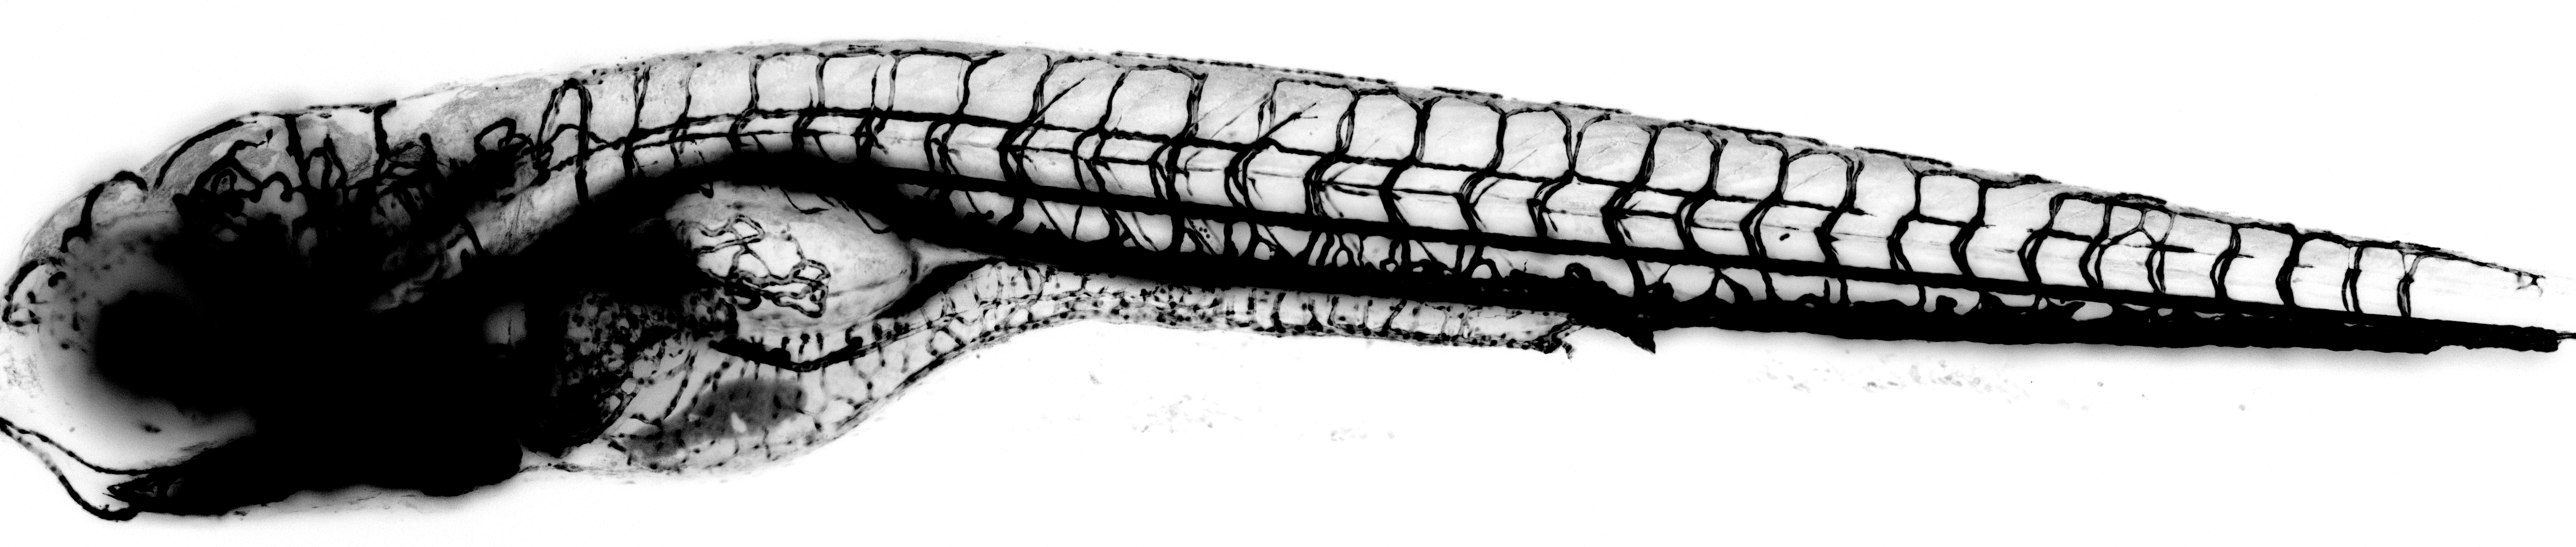
\includegraphics[width=\textwidth]{images/flk1gfp.png}
\caption[\textit{flk1}:\textit{eGFP\textsuperscript{s843}} larval zebrafish at 6 days post fertilization]{Black and white image of the \textit{flk1}:\textit{eGFP\textsuperscript{s843}} larval zebrafish, showing the regularly patterned intersomitic vasculature. This transgenic line allows for facile visualization and quantification of various angiogenic processes due to the highly stereotyped developmental patterns of the larval zebrafish endothelium.}
% Provide a label so we can cross\hyp{}reference it from the tex
\label{figure:flk1}
\end{center}
\end{figure}

The zebrafish is a powerful model for studying various aspects of vascular development and endothelial cell biology \citep{Wilkinson2014}. As we have already seen with the tale of the \textit{cloche} mutation, the zebrafish allows for sophisticated genetic and optical analysis of the fine details of vascular development. The zebrafish offers an array of benefits for the study of vascular processes including strong conservation of underlying genetic pathways, optical accessibility from the earliest events of development, oxygen perfusion by passive diffusion for most of the larval stages \citep{Ellertsdottir2010}, a superabundance of genetic tools (\autoref{figure:flk1}), and a highly stereotyped pattern of vascularization, from which even minor perturbations can be detected \citep{Jin2005}. These features and more make the zebrafish perhaps the gold\hyp{}standard model for studies of vascular patterning.

The biology of the zebrafish opens the possibility of studying processes in vascular development that are impossible to do in a viviparous animal. External fertilization and development makes it possible to precisely determine the stage at which vascular malformations induce developmental failure in a highly oxygenated environment. These things are possible to varying degrees in the mouse, for instance, but the number of replicates and the resolution of observation are unmatched in the zebrafish. 

Even the earliest events of vascular specification can be modeled in the zebrafish and translated essentially one\hyp{}to\hyp{}one into humans and zebrafish have been instrumental in identifying these cellular differentiation events that give rise to the earliest hemangioblasts and the consequences thereof. These hemangioblasts function as a bipotent lineage able to differentiate into both angioblasts and hematopoietic stem cells, generating the blood and lymphatic vasculature as well as all of the hematopoietic lineages \citep{Vogeli2006}. Angioblasts migrate individually toward the midline of the zebrafish and coalesce to form the dorsal aorta, a process that can be watched in real time with fluorescent imaging \citep{Lawson2002}. This early process is mediated by a short peptide and functions independently of VEGFA despite VEGFA being expressed by this point in development \citep{Nasevicius2000, Liang2001, Hogan2017}. At later points in development, cells along the dorsal aorta of the zebrafish larvae dedifferentiate and become the hemogenic endothelium, from which hematopoietic stem cells arise to see the development of myeloid and erythroid populations by approximately 24 hours post fertilization \citep{Gore2012}. 

Later steps depend on angiogenesis to form new blood vessels, a process intimately dependent on VEGFR signaling. In the absence of VEGFR, vascular sprouting is profoundly reduced and subsequent vasculature is malformed; this also suggests that there are some non\hyp{}VEGF cues that initiate angiogenesis but are unable to properly regulate it to generate a mature endothelial system \citep{Hogan2017}. These may be aberrant vasculogenesis efforts or angiogenesis induction by other mechanisms that will be discussed at greater length in further sections.

These developmental angiogenic processes have a great deal in common with the mechanisms underlying pathological angiogenesis, as highlighted in \autoref{angiogenesis}. During development, the somites of the zebrafish express Vegfaa to induce the formation of the stereotypic intersomitic vasculature that comprises the vascular patterning along the trunk; such developmental \textit{vegfaa} expression can be seen clearly in transgenic approaches to visualizing this pathway \citep{Karra2018, Walton2018}. Despite the central role of VEGFA in angiogenesis, there are other auxiliary factors that are also capable of inducing angiogenesis, including BMPs, plexins, Notch, and CXCR4. The role of CXCR4 has been discussed in \autoref{mamaw}, but in development this chemokine can guide endothelial migration to ensure proper vascular connections and proper physical differentiation of the blood and lymphatic vascular systems. This role for CXCR4 is thought to be in mediating migration of already active angiogenesis and not in the initiation stage \citep{Schuermann2014}.

An interesting aspect of vascular development that remains somewhat mysterious while also being a critical dimension of vascular\hyp{}targeting therapeutic strategies is the process of lumen formation within the growing vasculature. While the events of tip cell initiation, migration, and guidance have been detailed in some depth, the process of opening a lumen through which blood can flow is less well detailed, partially for lack of effective \textit{ex vivo} complementary strategies for study. One known mechanism for this is through vacuolar fusion between neighboring cells, making the entire vessel one cell in thickness with a hollow center running along the length of the structure \citep{Kamei2006}. Such a process might be expected to predominate in the long, thin vascular spindles seen in our model of zebrafish granuloma formation, although detailed analysis of the structural features of these vessels remains lacking.

The regularly patterned intersomitic vasculature of the larval zebrafish makes it an excellent platform to study the angiogenic potential of a vast range of possible stimuli. In my work, I have used this patterned region to measure perturbations in a highly sensitive manner, as has been done by other previously \citep{Oehlers2015, Walton2018}. The developmental regularity of this location offers many advantages for studying these processes and the area generally has only sparse macrophage residency at early points in development, allowing for some degree of macrophage recruitment and then angiogenesis to be experimentally studied. This location seems like a prime potentiator of future studies on pro\hyp{} and anti\hyp{}angiogenic drug screening given the ease with which stimuli can be implanted into the trunk of the larval zebrafish.

\subsection{Challenges in the Use of the Zebrafish Model}\label{zfchal}

While extremely powerful, the zebrafish is still not a perfect model; the model chosen to address any question must be the one that most clearly mirrors the process being examined (and, for the zebrafish in particular, the tools to address the question must exist within the model). Challenges with zebrafish can be summarized in four major issues: fish\hyp{}specific differences in biology, the aforementioned whole genome duplication, lack of true inbred models, and a lack of biochemical reagents to study zebrafish proteins.

The focus of this work is the study of tuberculosis disease, which in humans is a predominantly pulmonary infection that spreads from person to person via aerosolized droplets from the respiratory tract. Zebrafish, being fish, do not have lungs and are thus rendered impotent when it comes to the study of mycobacteria\hyp{}lung interactions, including those with alveolar macrophages. While the zebrafish faithfully recapitulates many aspects of tuberculosis disease and the shared genetic programs that drive macrophage immune responses, granuloma formation, angiogenesis, and host protection, any aspects that are specific to a given tissue may not be able to be captured with this model and other models should be employed in a complementary fashion to improve overall biological understanding. 

The ancestral whole genome duplication has resulted in both a great deal of redundancy within the zebrafish genome that requires much more exhaustive genetic work than the often one\hyp{}to\hyp{}one gene pairs in humans and mice. While this does not inhibit the potential for discovery, it increases experimenter labor and can slow progress as the ``functional'' ortholog is sought out of a potential set of partially homologous genes. On the other hand, the inverse can often occur -- unexpected roles for zebrafish proteins then translate into a shared function in the mammalian counterpart, which can typically only be discovered either incidentally or through unbiased screening approaches. This is not to suggest that such issues cannot occur in the mouse, as they have very famously with studies on DC-SIGN \citep{GarciaVallejo2013, Tanne2009} and IRGM \citep{Dockterman2022, Henry2009, Singh2010, Bekpen2009, Singh2006,Bekpen2010}, but that such issues tend to be more frequent and troublesome in the zebrafish model.

While the outbred nature of common laboratory zebrafish lines is an advantage in many respects, the lack of inbreeding fuels two issues: a poor quality reference genome and high degrees of heterogeneity within the population regarding particular responses, especially immune responses. The reference genome was a monumental effort and resulted in reasonable coverage across 1.4 gigabases \citep{Howe2013}. However, long regions of repeats and ambiguous calls along many introns have left it inferior to comparable mouse and human genomes, which were constructed from extremely laborious but precise bacterial artificial chromosome cloning and Sanger sequencing \citep{Osoegawa2000}. While the reference strains were derived from doubled haploid founders, there remains substantial genetic diversity within these so\hyp{}called strains\footnote{As detailed at \url{https://zfin.org/ZDB-GENO-960809-7}, the *AB zebrafish lineage is derived from an isolated but widely intercrossed set of lines without a dramatic series of bottlenecks to force true homozygosity (likely because this is impossible). The large numbers of offsprings and parents for each new generation ensures a relative degree of outbreeding that becomes obvious with further genomic studies \citep{Deng2022}.} \citep{Suurvali2020, Holden2018, Deng2022, ZFIN}. 

Lastly, the lack of antibodies available for the fish is a ubiquitous complaint among zebrafish researchers. While mice have $>$5000 antibodies available from Abcam and humans have nearly 20,000, zebrafish have 105 at the time of this writing in December 2022. While obviously not the full breadth of all available antibodies, it demonstrates the relative lack of these tools in the zebrafish, which inhibits protein localization studies in fixed tissue as well as a more trial\hyp{}and\hyp{}error approach to studying genes of interest. While the situation is steadily improving, what is needed is a community\hyp{}wide initiative to generate and share (ideally sequence\hyp{}defined, monoclonal) antibodies from a variety of host species against a range of proteins, ideally at highly conserved locations for use in other models. Such a resource would greatly accelerate discovery in the fish, but seems to be many years off, by which time, perhaps, new computational methods to antibody\hyp{}target binding will make the laborious process of host immunization and then affinity purification a moot point and enable a genetics\hyp{}first approach to antibody discovery \citep{Wilman2022, Hummer2022, Akbar2022a, Akbar2022b, Shan2022}. Libraries of camelid single domain antibodies are pushing ever\hyp{}closer to this elusive goal \citep{ValdesTresanco2022, Moutel2016}. A program comparable to AlphaFold able to predicting high-affinity binding to particular proteins would revolutionize all of biomedical science in a way that nothing else (including CRISPR and RNA-seq) have.

\section{\textit{Mycobacterium marinum}\hyp{}Zebrafish Model of Tuberculosis}\label{zfmm}

Work by the Ramakrishnan group, began in part in Stanley Falkow's lab, led to the development of a heterologous model system for the study of tuberculosis. \textit{M. tuberculosis} is an extremely slow\hyp{}growing pathogen\footnote{The doubling time is approximately 24 hours and the time to visualizable colonies is on the scale of three or four weeks.} that must be handled under biosafety level 3 (BSL\hyp{}3) conditions. These requirements make working with \textit{M. tuberculosis} challenging; deficiencies in the mouse model compound the issue and lead to difficulty in studying specific aspects of the host\hyp{}pathogen interface. Thus, the development of a complementary model able to facilitate visual access and that reproduces key aspects of the human disease had the potential to unlock new insights into these interactions and, over the past twenty years, have done precisely that \citep{Myllymaki2016}.

\subsection{History and Merits of the Zebrafish\hyp{}\textit{M. marinum} Model}\label{zfmmhis}

Studies began in the mid\hyp{}1990s set the stage for the emergence of a new model of tuberculosis infection. \citeauthor{Ramakrishnan1994} utilized a closely related pathogenic species of mycobacteria, \textit{Mycobacterium marinum} to demonstrate a temperature\hyp{}dependent persistence in cultured cells. A subsequent study found that \textit{M. marinum} was able to infect and cause consumptive disease in \textit{Rana pipiens} frogs as well as infect human extremities \citep{Ramakrishnan1997a, Ramakrishnan1997b, Cosma2006}. A new model was also developed using carp leukocytes, allowing macrophage\hyp{}mycobacterial interactions to be studied at BSL\hyp{}2 conditions \citep{ElEtr2001}. A foundational study in 2002 set the tone for the next two decades of research into host\hyp{}microbe interactions in the zebrafish. \citeauthor{Davis2002} took advantage of the optical transparency and manipulative amenability of the zebrafish larvae to infect them with \textit{M. marinum}. \textit{M. marinum} is a globally dispersed pathogen of fish and amphibians that causes tuberculosis in fish, which tends to manifest in superficial lesions, spinal deformities, and wasting and which can occasionally infect humans, typically on the superficial extremities where the body temperature is within the growth range of the bacterium \citep{Hashish2018, Aronson1926, Gray1990, Parisot1958}. The use of this heterologous host\hyp{}pathogen system allowed for the first ever \textit{in vivo} visualization of the early processes of granuloma formation through the interactions between the invading bacteria and the responding host macrophages, which serve as the first responding innate immune cells to mycobacterial infections \citep{Davis2002, Davis2009}. This ability to dissect the relative contributions of the innate immune system in an unmodified organism has enabled many studies on the specific roles of macrophages and neutrophils in host immune control and has highlighted the imminent importance of these early responses in infection control that had been ignored by the IFN\hyp{}$\upgamma$ and T cell\hyp{}biased control seen in C57BL/6 mouse models \citep{Lesley2008}.

Further developments over the following years, most notably by \citeauthor{Swaim2006} in 2006, established the zebrafish as a sophisticated and multifaceted model that allows for both comprehensive live imaging of the early processes of infection and dissection of the later stages of infection using adult zebrafish that form granulomas morphologically similar to those formed by humans in response to both \textit{M. tuberculosis} and during opportunistic infections by \textit{M. marinum}. These findings set the stage for the continued development of the zebrafish\hyp{}\textit{M. marinum} model of tuberculosis and has enabled the study of processes of human disease that have been long described but previously unable to be evaluated.

While a great deal was done to develop the model over time, there remained important questions about the ability for these findings to be translated into humans; mice are the preeminent preclinical model and to translate findings in the fish directly into humans could, in certain instances, dramatically cut the bench\hyp{}to\hyp{}bedside timeline. A pair of seminal papers \citep{Tobin2010, Tobin2012} established the \textit{LTA4H} locus as a major determinant of the course of tuberculous meningitis -- individuals with either homozygous allele were at increased risk of poor outcomes and treatment of one of the homozygous populations with dexamethasone was proposed as a host\hyp{}directed therapy to improve outcomes in this deadliest of tuberculosis manifestations. Indeed, subsequent studies found that this patient stratification strategy was able to determine patient response to dexamethasone in tuberculous meningitis \citep{Thuong2017, Thwaites2013, Wilkinson2017, Davis2018, Prasad2016}, although there may be additional factors worth considering beyond just \textit{LTA4H} genotype \citep{Siddiqi2021}.

Today, the zebrafish\hyp{}\textit{M. marinum} model continues to proliferate in utility and acceptance. Indeed, as the field of zebrafish research as a whole advances technologically, it allows the advantages of the fish to shine through even more so in the study of host\hyp{}pathogen interactions. New technologies for spatial transcriptomics will be greatly enhanced by our knowledge base in zebrafish development and the existing optical transparency of the larval fish; the day is likely not far distant when a comprehensive, spatially\hyp{}aware transcriptional atlas of the developing zebrafish larva will be available analogous to that of \textit{Caenorhabditis elegans}, which will only accelerate our knowledge of host\hyp{}tuberculosis dynamics through added dimensional awareness \citep{Packer2019}.

As alluded to, one of the most useful incidental features of the fish is the temporal segregation of innate and adaptive immune responses \citep{Myllymaki2016}. While the adult zebrafish possesses the complete vertebrate immune system, including both myeloid and lymphoid compartments, the larval zebrafish is limited to innate immune responses \citep{Cronan2014}. This allows the researcher to differentiate the contributions of these two distinct systems to the overall phenotype and to, in an unmodified host, ascribe discrete roles to the innate immune system. This is one of the major reasons why so much has been learned about macrophage\hyp{}mycobacterial interactions using the larval zebrafish -- it allows for analysis of these interactions in the context of a native, immunocompetent host but without confounding intervention from adaptive immunity.

\subsection{Zebrafish Husbandry}\label{husbandry}

Zebrafish husbandry serves as one of the major advantages of the model. Social fish, they can be maintained at a reasonably high density per unit volume as adults\footnote{Approximately 250 mL of water per fish is more than sufficient for rapid growth to adulthood and breeding success.}, which can then spawn ${\sim}$200 eggs per week per female. Our fish are kept on a constantly recirculating rack system from Aquaneering, which replaces 90\%+ of the volume of each of ${\sim}$1,000 tanks once per hour, 24 hours a day. The fish are diurnal animals and seasonally-indifferent photoperiodic breeders, which greatly eases experimenter access, as they will reproduce reliably only in the morning, which can be artificially set to the convenience of the laboratory. The fish are kept at 28.5$^{\circ}$C on a 14hr\hyp{}10hr light\hyp{}dark cycle and kept in either 3 or 6 L tanks. Reverse osmosis water is maintained at 600\hyp{}700 $\upmu$S conductivity by addition of Instant Ocean Sea Salt (\#SS15\hyp{}10) and a pH between 7.0 and 7.4 (buffered by automated addition of sodium bicarbonate; Arm \& Hammer Pure Baking Soda [\#426292]). All of this work was performed in accordance and compliance with policies approved by the Duke University Institutional Animal Care and Use Committee (protocol \#A091\hyp{}20\hyp{}04).

Infected adult zebrafish are maintained at an identical 14hr\hyp{}10hr light cycle at 28.5$^{\circ}$C in an isolated incubator (ThermoFisher \#PR505755L) physically separated from the primary fish system. Fish are kept at no greater than 1 fish/100 mL of water in Aquaneering crossing cages (Aquaneering \#ZHCT100) and are fed daily with the standard fish diet in our lab (Skretting \#GEMMA Micro 500). Water is changed daily using water taken from the primary fish system. While sex is not a standard factor we account for in the analysis of our experiments, approximately equal numbers of fish of each sex are used for infection experiments. Any adult fish exhibiting signs of imminent distress or morbidity\footnote{inability to right, flared scales, labored breathing, obvious open wounds} are euthanized. Standard adult experiments are conducted for a minimum of 14 days, although infection will continue to progress over the course of approximately four to six weeks if needed. Fish are humanely euthanized at the conclusion of experimentation by tricaine overdose and decapitation.

For infection, fish were anesthetized in 120 $\upmu$g/mL tricaine. Single\hyp{}use aliquots of single cell suspensions of \textit{M. marinum} were thawed and diluted in sterile PBS and zebrafish were injected with 10 $\upmu$L of a solution containing 200\hyp{}1000\footnote{While the precise number is kept consistent within each experiment and subsequent replicates, different initial inocula are chosen based on the desired kinetics of disease. Lower initial doses are likely to be superior for identifying factors regulating bacterial control while higher doses are better if the desired outcome is to study aspects of granuloma biology, as high starting doses tend to result in a greater number of granulomas forming earlier in disease. This often appears to balance out as the disease progresses and some functional upper limit on bacillary load is reached.} fluorescent bacteria using a back\hyp{}loaded insulin syringe (BD \#08290\hyp{}3284\hyp{}38). Injection is done into the peritoneal cavity of the fish, achieving a systemic infection within the cavity and which spreads to all major organ systems\footnote{Although brain involvement is only rarely seen. It is not a standard tissue for us to analyze in the lab, but previous analysis has generally failed to identify meningitis as a manifestation of \textit{M. marinum} infection in the zebrafish.}. 

The larval zebrafish, on account of the high fecundity of the model, is a key tool in these studies. We can readily collect $>$1,000 embryos at once and can reasonably infect ${\sim}$200 per hour, allowing for high n\hyp{}value screening approaches. This, in addition to their remarkable ability to recover and highly stereotyped developmental patterning, facilitates reproducible studies in many fields of biology including the work described herein. Embryos are collected in the early\hyp{} to mid\hyp{}afternoon and allowed to develop in the presence of 0.001\% methylene blue in E3 medium (5 mM NaCl (Fisher Scientific \#S271), 178 $\upmu$M KCl (VWR \#BDH9258), 328 $\upmu$M CaCl2 (VWR \#BDH9224), 400 $\upmu$M MgCl2 (Ward's Scientific \#470301)) at no more than 150 larvae per dish. At 24 hours post fertilization, they are transferred into E3 supplemented with 1\hyp{}phenyl\hyp{}2\hyp{}thiourea\footnote{The ability to taste phenylthiourea (also known as phenylthiocarbamide) is an interesting genetic trait in humans that can predispose individuals to enjoying the taste of various cruciferous vegetables \citep{Kim2003}.} (PTU, Sigma\hyp{}Aldrich \#P7629) at a final concentration of 45 $\upmu$g/mL to prevent melanization if they are to be used for imaging studies. Otherwise, they are allowed to develop in unmodified E3 medium until 3\hyp{}4 days post fertilization, when they are put into the nursery system to be raised to adulthood. Infected larval zebrafish are euthanized prior to 8 days post fertilization in all instances. Zebrafish are of indeterminate sex\footnote{This is only strictly true for laboratory strains of zebrafish \citep{Kochakpour2008}. Wild zebrafish have a sex determining region on chromosome 4 that has been repeatedly lost under laboratory culture conditions, for reasons that remain mostly unknown \citep{Howe2013, Parichy2015, Wilson2014}. In the lab, a variety of factors seem to influence the eventual sex determination of the fish, including rearing density and caloric allotment, in addition to various genetic factors \citep{Kossack2019}. Despite the lack of strict genetic determinants of sex, the standard 1:1 female:male ratio is generally maintained under normal conditions.} until they reach the juvenile stage of development, so no distinctions are or can be made on the basis of sex in larval zebrafish studies.

For ease of manipulation and the minimization of distress, larval zebrafish are anesthetized in approximately 160 $\upmu$g/mL of tricaine (MS\hyp{}222 or Tricaine\hyp{}S\footnote{Now known as ``Syncaine''}, Syndel \#ANADA 200\hyp{}226) prior to injection. Injection of \textit{M. marinum} is done by injecting larvae into a developmentally undefined peri\hyp{}notochordal space between the somitic muscle layers along the trunk at 2 days post fertilization. Approximately 50\hyp{}150 fluorescent bacteria are injected, spreading along the anterior\hyp{}posterior length of the fish and establishing a largely localized infection along the avascular trunk. This infection location allows for facile quantitation of vascular aberrations, an essential prerequisite for this study. Injection of TDM is conducted similarly. Trehalose 6\hyp{}6'\hyp{}dimycolate from \textit{Mycobacterium bovis} (TDM, Sigma\hyp{}Aldrich \#T3034) was resuspended in 2:1 v/v chloroform:methanol at 1 mg/mL and stored at \hyp{}80$^{\circ}$C. Prior to use, the liquid is evaporated under vacuum and emulsified in incomplete Freund's adjuvant (IFA, Sigma\hyp{}Aldrich \#F5506) at 2 mg/mL. Larvae are then anesthetized and injected with approximately 10\hyp{}20 nL of TDM/IFA or IFA alone along the trunk in this same undefined peri\hyp{}notochordal space. The droplets coalesce into spheres within 10\hyp{}15 minutes and remain in place for the entire experimental duration. Larvae are allowed to recover in E3 medium supplemented with PTU and raised in a 28.5$^{\circ}$C incubator.

Images were captured on a Zeiss Z1 compound epifluorescent microscope and processed in FIJI/ImageJ. The Z stacks were panned across to identify aberrant vasculature, which was then traced using the "Segmented Line" tool. This was used to capture the length to a Results Table, which was then used for subsequent analysis and plotting.

\begin{code}
\caption{This is a reference model for the analysis used to evaluate differences in angiogenesis across different genetic and treatment groups. In all instances, raw vascular measurements from FIJI/ImageJ are imported, paired with a key file (either genotype or file name depending on blinding strategy), and then plotted with ggplot.}
\label{zebrafishanalysis}

\inputminted[breaklines,frame=single,fontsize=\small]{r}{source/fish_plot_example.R}

\end{code}

\subsection{Deficits of Mouse Models of Tuberculosis}\label{mouse}

One model in particular, the C57BL/6 \textit{Mus musculus} mouse model, has become a ubiquitous feature of every major research institution all over the world due to their clonal nature\footnote{Genetic diversity between individual C57BL/6 mice is in the range of 10\hyp{}20 single nucleotide polymorphisms per individual in a genome of 2.5 gigabases -- a remarkable degree of isogenicity \citep{Bryant2011, Sarsani2019}.}, relative ease of use, and minimal expense\footnote{A single C57BL/6 mouse from Jackson Laboratories (jax.org) at the time of writing is \$24 USD.}. However, their genetic homogeneity fails to reproduce many phenotypes seen in human disease, making them an excellent model for some disorders and an insufficient one for others. Such loss of heterozygosity far from models the human condition, where there are an estimated 20 million base pairs of difference from person to person \citep{Genomes2015}. The difficulties of the mouse model are nowhere more apparent than in developmental biology. Although mouse viviparous development is extremely well defined and stereotyped over the course of gestation, that is precisely the challenge. Gestation is an internal and ongoing process of physiological and anatomical development and while it is possible to catalog the process of development in snapshots in time through vivisection, it is impossible to understand the kinetics and processes of development using a model that does not allow for immediate visual accessibility. While mice faithfully recapitulate certain aspects of human development, it is far from perfect and other approaches are able to access different types of knowledge in greater detail.

The mouse has served as the model for immunology for the past 50 years. It has enabled monumental discoveries that have resulted in new medications and therapies to treat nearly every conceivable human disease and is the foundation of every single chemotherapeutic medicine on the market today. The diminutive mouse is an outstanding model for a vast array of human diseases and continues to be the go\hyp{}to model for many processes and disorders. However, classical inbred mouse models, including C57BL/6 and other popular lines, including BALB/c, A/J, and 129S1, fail to replicate defining characteristics of tuberculosis in ways that compromise our ability to apply findings from these models to the kinetics and pathology of human disease. For instance, the C57BL/6 mouse is highly resistant to acute tuberculosis disease; these mice can be infected with standard laboratory strains of \textit{M. tuberculosis} and succumb approximately 300 days later\footnote{Bacterial strain variations and dosage can alter this somewhat, but infection with the reference strain H37Rv will result in a highly reproducible and sudden series of death almost a year after initial infection.}.

Historically, the C57BL/6 mouse model of tuberculosis has served as the gold standard for studies on host\hyp{}pathogen interactions in tuberculosis and has been used to identify major host\hyp{}protective factors as well as bacterial virulence factors. However, even among other mouse models, the C57BL/6 model has clear challenges in the field of tuberculosis biology. For one, C57BL/6 does not form necrotic granulomas under standard laboratory doses of laboratory strains of \textit{M. tuberculosis} \citep{Orme1998}. This discordance between the observed human phenotype and the mouse model leaves an abundance of room for misinterpretation of data that may or may not be translatable to the human disease context. The loci of infection in this mice becomes a granulocytic infiltrate, with abundant cellular involvement and engagement with the bacteria, including the presence of lymphocytes \citep{Ulrichs2006, Hunter2007}. One of the standard arguments that the granuloma has host\hyp{}detrimental aspects is that the physical structure blocks T cell\hyp{}mycobacteria interactions, which may be able to serve an important host\hyp{}protective role. That this is incapable of being modeled in the C57BL/6 model leaves room for competing models to model these elements of granuloma biology.

More recently, the C3H/FeJ ``Kramnik'' mouse model has come into widespread use. This model is able to model granuloma biology, as ${\sim}$50\% of infected mice will form granulomas \citep{Harper2012, Lenaerts2015}. However, this is also a hypersusceptible model of infection, with the average mouse succumbing to infection within approximately 3 months. In humans, disease progression can be of either very rapid progression over the course of weeks or develop in severity over the course of many years \citep{Tiemersma2011}. An alternative model has been developed through knockout of \textit{Sst1}, which results in increased granuloma-like morphology in the mouse, but this has only been investigated in \textit{Mycobacterium avium} models of infection \citep{Rosenbloom2021}. Thus, there remains an unmet need for a model that (a) forms granulomas and mirrors other important aspects of human disease and (b) exhibits a spectrum of disease presentation similar to that seen in humans. 

Other mouse models could potentially fulfill some of these demands, if appropriately chosen. One approach has been to more precisely mimic the infectious trajectory of human disease by instilling mice with ultra\hyp{}low doses of \textit{M. tuberculosis} by aerosol, which seems to facilitate a more necrotic granuloma phenotype, perhaps suggesting that the previously used larger doses (${\sim}$300 CFU) were inducing a distinct immune response that led to more granulocytic infiltration \citep{Plumlee2021}. Recently, work by Clare Smith from the Sassetti lab has established the collaborative cross mouse collection as a fruitful tool for the discovery of novel aspects of host immunity to tuberculosis, including IFN\hyp{}$\upgamma$\hyp{}independent defense, the role of important T cell integrins, and more across approximately 50 inbred\hyp{}to\hyp{}homozygosity mouse strains \citep{Smith2016, Smith2022}. Further and ongoing dissection of these strains will not only reveal further determinants of host immunity and bacterial susceptibility, but may provide the elusive granuloma mouse model, although what factors render most mice incapable of forming human\hyp{}like caseating granulomas remains unknown; these host determinants of granuloma formation are also intriguing aspects of this axis that may reveal new contributions from genes of previously unknown function. However, the process of granuloma formation is one of synthetic tone -- the overall response itself may be more important than the contribution of any one factor, aside from major basal determinants, like STAT6 signaling \citep{Cronan2021} and some modicum of host defense through major immunostimulatory cytokines \citep{Flynn1993, Flynn1995}. In the long term, as understandings of the host determinants of granuloma formation are better understood, knock\hyp{}in and humanized models may provide an excellent means of modeling granulomas in the mouse but this seems like a far distant development that will require a great deal of work in the meanwhile to clarify the contributions of these diverse factors.

\subsection{Comparison to Other Models}\label{zfcomp}

Other popular laboratory models of tuberculosis are able to form granulomas, including rabbits and guinea pigs; the former is relatively resistant to tuberculosis while the latter is highly susceptible \citep{Clark2014, Dorman2004, Heppleston1949}. However, these tend to require maintenance via relative outbreeding, are larger mammals with associated higher husbandry costs, and are devoid of most useful genetic tools. This left a clear gap in our ability to understand some of the aspects of this important human disease that required innovative new approaches and a whole new paradigm. Additionally, these models do not escape the challenges of working in a BSL\hyp{}3 environment with \textit{M. tuberculosis}. While the cynomolgous macaque model of tuberculosis is an excellent representation of human tuberculosis, the costs associated with the use of macaques is enormous \citep{Pena2015}. A cost\hyp{}efficient, genetically amenable small vertebrate model of infection was a clear gap in the resources available in the late 1990s and the zebrafish was able to fill some of these gaps in our ability to model these infectious processes. As time has progressed, our ability to use the zebrafish to model different aspects of mycobacterial infection has expanded, with the zebrafish now able to be used for studies in \textit{M. leprae}, an incorrigibly difficult organism to study due to its peculiar lifestyle and agonizing doubling time ($\sim$12 days) \citep{Madigan2017} and \textit{M. abscessus}\footnote{The treatment of these non-tuberculous mycobacteria is a fascinating tale in the innovation of novel therapeutic approaches in patients with extensively drug resistant strains of these species. Recent studies have applied mycobacteriophages derived from the SEA-PHAGE project, an undergraduate-driven research project collecting environmental phages able to infect \textit{M. smegmatis}, to selectively infect and kill \textit{M. abscessus} \citep{Jordan2014, Dedrick2022, Dedrick2021, Dedrick2019}. The ability to leverage a science education effort in SEA-PHAGES to uncover therapeutic phages able to save lives is an incredible testament to the power of basic science to lead to unexpected clinical breakthroughs and sets forth a model for the discovery of additional mycobacteriophages that might be able to similarly treat drug-resistant tuberculosis.}, a close relative of \textit{M. marinum} \citep{Halloum2016, Stinear2008, Bryant2016}.

\section{Transgenic Tools in the Zebrafish}\label{transgenics}

Since that first monumental forward genetic screen in 1996, the arsenal of tools available to the zebrafish researcher has expanded dramatically. This expansion began rather soon thereafter, with a major \textit{insertional} mutagenesis screen being published, which allows for more rapid barcoding and identification of the disrupted gene than earlier ethylnitrosourea mutagenesis approaches \citep{Amsterdam1999}. Additionally, the ability to inject plasmid DNA and express exogenous constructs in the fish was discovered relatively early on \citep{Stuart1988, Lele1996}, but was extremely laborious in both time investment and effort required. The race was on for a technology that would be able to introduce DNA into the zebrafish embryo that would efficiently transmit across generations. The results of these labors were two complementary technologies: I\hyp{}SceI meganuclease\hyp{}mediated transgenesis \citep{Thermes2002} and \textit{tol2}\hyp{}mediated transgenesis \citep{Kwan2007}. I\hyp{}SceI transgenesis utilizes a ``meganuclease'' that recognizes and cleaves a specific, 18 base pair sequence only known to exist in the \textit{Saccharomyces} mitochondria. This, coupled with some useful biophysical properties, allows it to protect foreign DNA within cells until it can interact and integrate with the genome \citep{Soroldoni2009, Grabher2004}. While other approaches were attempted, including the use of retroviruses \citep{Kurita2004}, nothing else matched this system for ease of use and efficacy. However, research in medaka had begun utilizing transposons to mediate transgenesis to great effect and this was viewed as the future. Sleeping Beauty was an early attempt, but has largely fallen into disuse \citep{Davidson2003}, while \textit{tol2}, with its large cargo capacity \citep{Balciunas2006}, has become the dominant mode, largely thanks to the tol2kit, which is a Gateway\hyp{}cloning compatible kit of promoter, gene, and 3' UTR elements that can be used to rapidly clone components to generate transgenic zebrafish -- conceptualization to injection can be streamlined into ten days or less if needed \citep{Kwan2007}. This method was used in this work to generate the major new transgenic lines that enabled the work in \autoref{chap3}\footnote{I have, however, adapted the \textit{tol2} destination vector used throughout this work, pDEST tol2 Ubb pA, to an I\hyp{}SceI\hyp{}compatible destination vector for use with that system. The cloning steps are identical to the \textit{tol2} vector. This vector was created by two step PCR amplification of the ccdB/CmR cassette and the backbone. The ccdB/CmR cassette was amplified with \seqsplit{5'\hyp{}ACCGGTGGGAGGCGTTCGGGCCACAGCGGGACCATGATTACGCCAAGC\hyp{}3'} and \seqsplit{5'\hyp{}GACGTCTAGGGATAACAGGGTAATTGGTACCGTAAAACGACGG\hyp{}3'} while the backbone was amplified with \seqsplit{5'\hyp{}GACGTCCCGCTGTGGCCCGAACGCCTCCCGCATCAGCGCAATTCAATTGG\hyp{}3'} and \seqsplit{5'\hyp{}ACCGGTATTACCCTGTTATCCCTAGCAGGATAAAACCTTGTATGC\hyp{}3'}. These fragments were then digested with AgeI\hyp{}HF (NEB \#R3552L), AatII (NEB \#R0117L), and DpnI (NEB \#R0176L), heat\hyp{}inactivated, and ligated together with T4 DNA ligase (NEB \#M0202S) to produce pDEST I\hyp{}SceI Ubb pA.}.

Newer technologies are making the zebrafish ever\hyp{}more amenable to genetic manipulations and optical control. For a more in\hyp{}depth analysis of the state and future of genetic tools in the zebrafish, see \autoref{newtech}. The current range of tools available in the zebrafish is vast and able to specifically dissect key aspects of the host\hyp{}pathogen interface and new tools are released all the time. For instance, it is possible to drive the expression of multiple individual proteins off of a single polycistronic transcript through the use of 2A peptides \citep{Kim2011}. Relevant to the studies to come is the ability to visualize changes in calcium, which can be seen using calmodulin\hyp{}modified green and red fluorescent proteins known as genetically encoded calcium indicators, the most notable of which being GCaMP and its many variants \citep{Nakai2001, Dana2016, Zhang2021b}. These have be used to both measure and manipulate calcium flux in cells to alter their movement and immune responses \citep{Beerman2015}. The zebrafish offers the possibility to do calcium imaging across the entire larva at high spatial resolution, especially through use of newer microscopy techniques like LightSheet \citep{Reynaud2008, Kim2017}.

An additional tool is the use of gene trapping techniques, that insert either transcriptional repressors or polyadenylation sequences into genes and allow for these to be rescued through use of Cre or other methods. These have allows for various tagging approaches and have generated libraries of strains with fluorescence driven off endogenous promoters. Conversely, by placing native genes under the control of inducible promoters, it is possible to determine temporal effects of particular genes during development \citep{Ma2017}. These tools and others to be discussed later offer the opportunity to study the mechanisms of NFAT activation and the biology of these proteins in their native context. An \textit{nfatc2a} gene trap line would be ideal, but none has yet been identified \citep{Ichino2020, Clark2012}.

\subsection{Technical Description of New Transgenic Lines}\label{transtech}

The p5e \textit{irg1} construct was generated by restriction digestion of irg1\hyp{}pTol2linkerswitch \citep{Sanderson2015} (a gift from Christopher Hall) with FseI and XmaI and then blunted using T4 DNA polymerase (NEB \#M0203S) per the manufacturer's instructions. Simultaneously, p5e MCS \citep{Kwan2007} was PCR linearized using inverted T3 and T7 promoter primers (\seqsplit{5'\hyp{}CCCTATAGTGAGTCGTATTAC\hyp{}3'}, \seqsplit{5'\hyp{}TCCCTTTAGTGAGGGTTAAT\hyp{}3'}), digested with DpnI and PCR purified. These fragments were then ligated using T4 DNA ligase (NEB \#M0202S) to generate p5e \textit{irg1}. This plasmid was then recombined with pME tdTomato (Addgene \#135202), p3e \textit{ubb} pA (Addgene \#188702), and pDEST tol2 \textit{ubb} pA (Addgene \#188701) by Gateway cloning (ThermoFisher \#12538120) to generate the pTol2 \textit{irg1}:tdTomato construct that was then injected into single cell embryos alongside 15 ng/$\upmu$L \textit{tol2} mRNA (Balciunas et al., 2006) in 1x Tango buffer (ThermoScientific \#BY5). Candidate founders were selected based on fluorescence at 3 dpf, raised to adulthood, and outcrossed to *AB to establish the line, which transmits at $\sim$50\% frequency, suggesting a single insertion locus and has exhibited stable expression over ${\sim}$6 generations.

Tg(\textit{irg1}:\textit{VIVIT\hyp{}tdTomato\textsuperscript{xt38}}), in which the NFAT inhibitory peptide VIVIT conjugated to the fluorescent protein tdTomato is expressed strictly in macrophages, was constructed by recombination of p5E \textit{irg1} (Addgene \#188698), pME VIVIT NS (Addgene \#188699), p3E tdTomato (Addgene \#188700), and pDEST tol2 \textit{ubb} pA (Addgene \#188701). Reactions were incubated at equimolar ratios overnight in a 25$^{\circ}$C thermocycler with heated lid, with volumes calculated using the ``LR Ratios Calculator'' Excel document \citep{NFATZenodo}. The \textit{irg1} promoter was first described by Sanderson et al. as a macrophage\hyp{}specific inducible promoter, but our lab has found that this element often drives basal expression in macrophages as well, likely in an insertion\hyp{}site\hyp{}dependent manner\footnote{\textit{irg1}, or \textit{acod1} is an aconitate dehydrogenase that is specifically induced within macrophages by interferon responses. While we generally use this as a tool to mark macrophage populations, there is interesting biology related to the product of aconitate dehydrogenase, itaconate. The roles of itaconate in infection are many and will be explored further in \autoref{metabolism} \citep{Coelho2022, Peace2022, Lin2021, ONeill2019, Chen2022, Nair2018, Wu2020}.}. Tg(\textit{irg1}:\textit{tdTomato\textsuperscript{xt40}}) was similarly generated by recombination of p5E \textit{irg1}, pME tdTomato, p3E Ubb pA, and pDEST tol2 Ubb pA. Both of these lines express tdTomato at baseline within macrophages by 48 hours post fertilization.

The development of Tg(\textit{lyz}:\textit{VIVIT-tdTomato\textsuperscript{xt39}}) was conducted similarly, replacing p5e \textit{irg1} with p5e \textit{lyz} \citep{Hall2007}. These fish were injected at the single-cell stage and screened for tdTomato expression at 2 days post fertilization. Positive founders were raised to adulthood and screened for transmission. A single founder was identified that transmitted at $\sim$50\% frequency and these were then used to further establish this transgenic line, which has sustained stable expression over approximately 4 generations.

The middle element, pME VIVIT NS was constructed by a synthetic templated PCR after annealing. Two oligonucleotides from Integrated DNA Technologies (IDT) were annealed by heating to 95$^{\circ}$C and then slowly cooled to room temperature (sense: \seqsplit{5'\hyp{}GCCATCATGGCAGGACCACACCCGGTGATTGTTATCACTGGACCACATGAGGAG\hyp{}3'}, anti\hyp{}sense: \seqsplit{5'\hyp{}CTCCTCATGTGGTCCAGTGATAACAATCACCGGGTGTGGTCCTGCCATGATGGC\hyp{}3'}). This was then used as a template for PCR using two primers to add the \textit{attB1} and \textit{attB2} sites required for Gateway recombination into pDONR 221 (forward: \seqsplit{5'\hyp{}GGGGACAAGTTTGTACAAAAAAGCAGGCTGCCATCATGGCAGGACC\hyp{}3'}, reverse: \seqsplit{5'\hyp{}GGGGACCACTTTGTACAAGAAAGCTGGGTACTCCTCATGTGGTCCAGTG\hyp{}3'}). This PCR product was then column purified and recombined into pDONR 221 (ThermoFisher \#12536017) using BP Clonase II (ThermoFisher \#11789020) to generate pME VIVIT NS (no stop) (Addgene \#188699). Constructs were verified by either Sanger sequencing or whole plasmid sequencing from Plasmidsaurus and have been submitted to Addgene, which provides additional whole plasmid sequencing verification.

Genotyping to differentiate the \textit{irg1}:\textit{tdTomato\textsuperscript{xt40}} and \textit{irg1}:\textit{VIVIT\hyp{}tdTomato\textsuperscript{xt38}} lines can be performed where necessary (either for intentional experimental blinding or due to incidental mixing of fish during husbandry or experimentation) by PCR and gel electrophoresis. Primers (\seqsplit{5'\hyp{}GATTTAGGTGACACTATAGATTCAGAGCTCGCACAGG\hyp{}3'}, \seqsplit{5'\hyp{}ATCTCGAACTCGTGGCC\hyp{}3'}) amplify across the 3' end of the \textit{irg1} promoter and into the 5' end of the tdTomato insert. VIVIT+ fish display a 236 bp band while tdTomato\hyp{}only fish display a 163 bp band. No band is seen in sibling fish lacking an \textit{irg1} transgene. 

\section{Use of CRISPR/Cas9 in Zebrafish}\label{crispr}

One of the major advantages of the zebrafish model is that, unique among vertebrate model organisms, it is trivial to generate targeted knockouts of essentially any gene using CRISPR/Cas9, which can be performed by even new researchers in the course of a couple of hours. Compare this to the mouse where it takes highly technical single cell injection and implantation to screen for new lines, which can often cost thousands of dollars to outsource. Extensive work has been done to establish different applications of this technology to generate F\textsubscript{0} individuals for high\hyp{}throughput screening, knock\hyp{}in technology to use endogenous promoters and tag genes, whole\hyp{}segment deletions for total gene removal, and more. 

One of the huge advantages of CRISPR/Cas9 in zebrafish is the ability to use ``crispants'' to assess phenotypes, which is very rapid and allows for efficient screening of different genes than the standard injection, rearing, and isolating single heritable mutations pipeline. This approach has been extensively studied and described elsewhere, but with the correct approach, these results often faithfully recapitulate phenotypes seen in stable mutants \citep{Zhang2017, Wu2018}. This approach transforms six months of waiting into as little as a week from injection to preliminary data -- a huge time savings that allows for more informed experimentation.

Generation of mutants in \textit{myd88}, \textit{card9}, \textit{nfatc2a}, \textit{nfatc3a}, ENSDARG00000079903, ENSDARG00000077975, and ENSDARG00000056379 was performed as described previously \citep{MorenoMateos2015}. Briefly, the oligonucleotides produced by CRISPRscan were utilized as a PCR template paired with the common sgRNA tail oligo (\seqsplit{5'-AAAAGCACCGACTCGGTGCCACTTTTTCAAGTTGATAACGGACTAGCCTTATTTTAACTTGCTATTTCTAGCTCTAAAAC-3'}). These were mixed at equimolar ratios (5 $\upmu$L each from 10 $\upmu$M stocks) into a standard Q5 (NEB \#M0491S) reaction mixture containing 2x concentration of dNTPs (NEB \#N0447S) and thermocycled using the following parameters: 98$^{\circ}$C -- 30 sec, [98$^{\circ}$C -- 5 sec, 45$^{\circ}$C -- 30 sec, 72$^{\circ}$C -- 15 sec] x 24, 72$^{\circ}$C -- 5 min, 4$^{\circ}$C -- $\infty$. This product was then PCR purified using a commercial kit by the manufacturer's instruction (Macherey-Nagel \#740609). This product was then used in an \textit{in vitro} transcription reaction using the NEB T7 HiScribe kit (NEB \#E2040S) with the following adjustments: 17 $\upmu$L template, 2 $\upmu$L GTP, 2 $\upmu$L CTP, 2 $\upmu$L ATP, 2 $\upmu$L UTP, 2 $\upmu$L enzyme, 3 $\upmu$L buffer and left to react overnight at 37$^{\circ}$C. This was then purified using the Monarch Total RNA Miniprep kit (NEB \#T2010S). RNA was diluted to 500 ng/$\upmu$L in TE and stored at \hyp{}80$^{\circ}$C until use. On the morning of injection, 1 $\upmu$L of RNA was added to 1 $\upmu$L of 63 $\upmu$M recombinant Cas9 protein (IDT DNA \#1081059) in 1x Tango buffer (ThermoFisher \#BY5). This mixture was then injected into single cell embryos and these were then either used directly for experiments or raised to adulthood to be screened as potential founders. Alleles were identified by outcrossing of mosaic adults to wild\hyp{}type *AB and Sanger sequencing of F\textsubscript{1} adults. DNA extraction was conducted by cellular lysis in 50 mM sodium hydroxide as described previously (Meeker et al., 2007). Briefly, either adult zebrafish tail fins or whole larvae were collected in 50 mM NaOH in H\textsubscript{2}O and lysed at 98$^{\circ}$C for 12 minutes in a thermocycler and then neutralized by 1:10 addition of a solution of 1M Tris\hyp{}HCl (pH 8) in 10x TE (100 mM Tris, 10 mM EDTA). This solution was then directly used as the template for downstream PCR reactions. 

Once a mutation has been established, efficient and cost\hyp{}effective genotyping is essential for differentiating the different genotypes. High\hyp{}throughput and researcher blinding are also important dimensions in this and one major method of blinded genotyping at scale is via high\hyp{}resolution melt analysis, or HRMA. HRMA utilizes a qPCR\hyp{}based amplification with a super\hyp{}saturating concentration of dsDNA\hyp{}binding dyes to sensitively detect changes in the thermal melting profile of DNA \citep{Reed2007, Thomas2014}; changes in the base\hyp{}pair composition will alter the melting profile of the DNA. While larger mutations are generally easier to differentiate, this assay can theoretically detect changes as small as a A/G or C/T transition, but is often limited by the detection precision of the instrument. We have thus employed a streamlined combination of the described rapid and efficient DNA extraction via alkaline lysis \citep{Meeker2007} with HRMA for the purposes of genotyping at every possibility. Other methods are only utilized if HRMA has failed, thus the use of classical PCR and restriction digestion to genotype \textit{nfatc2a} mutants.

The allele \textit{myd88\textsuperscript{xt29}}\footnote{This allele was originally published in \fullcite{Walton2018} and was generated by Rebecca Beerman.} was generated by injection of a single guide RNA into single-cell embryos (guide sequence: \seqsplit{5'-TAATACGACTCACTATAGGCGGCAGACTGGAGGACAGGTTTTAGAGCTAGAA-3'}). Adult zebrafish derived from the injected embryos were crossed to wild-type fish, and the progeny were assessed via HRMA as described previously. F primer: \seqsplit{5'-CCGAAAGAAACTGGGTCTGTTCC-3'}; R primer: \seqsplit{5'- ACGAGTTTCCCAGTCCGTCA-3'}. Larvae exhibiting lesions at the \textit{myd88} target locus were further analyzed by sequencing, and an allele exhibiting a 22 bp deletion was identified. This deletion begins at amino acid 39 (of 284) and results in a frameshift and premature translation termination after 59 amino acids. F\textsubscript{1} adult fish heterozygous for this allele were identified and pooled, and larvae used for the experiments requiring myd88 knockouts were generated by crossing these F\textsubscript{1} adults in the \textit{flk1}:\textit{eGFP} background. The resulting progeny exhibited Mendelian ratios of homozygous wild-type, heterozygous mutant, and homozygous mutant alleles via HRMA.

The allele \textit{card9\textsuperscript{xt31}} was generated by injection of a single guide RNA into single\hyp{}cell embryos (guide sequence: \seqsplit{5'\hyp{}TAATACGACTCACTATAGGGCAAGGTGCTGAGCAGCGGTTTTAGAGCTAGAA\hyp{}3'}). We identified an allele containing a 28 bp insertion, resulting in an immediate downstream frameshift leading to a premature termination codon at amino acid 59 (with missense mutations beginning at amino acid 47). Genotyping was performed using high\hyp{}resolution melt analysis (HRMA) using the MeltDoctor Master Mix (Applied Biosystems \#4415450) with primers flanking the sgRNA site (\seqsplit{5'\hyp{}CCTTATCTGAGACAGTGCAAGGTGC\hyp{}3'}, \seqsplit{5'\hyp{}TTACCAACTTTGCGGCGTCTG\hyp{}3'}). Amplification for Sanger sequencing was performed using primers (\seqsplit{5'\hyp{}GTTTTCCCAGTCACGACCGAATGCTTCTCATCAAGACC\hyp{}3'}, \seqsplit{5'\hyp{}CGAATGCTTCTCATCAAGACC\hyp{}3'}. Sequencing was performed with the ``M13F(\hyp{}40)'' primer from Eton Biosciences (\seqsplit{5'\hyp{}GTTTTCCCAGTCACGAC\hyp{}3'}).

The allele \textit{nfatc2a\textsuperscript{xt69}} was generated by simultaneous injection of two neighboring guide RNAs to increase odds of a larger intervening deletion (guide sequences: \seqsplit{5'\hyp{}TAATACGACTCACTATAGGGCTGCGAGAACGGGCCACGTTTTAGAGCTAGAA\hyp{}3'}, \seqsplit{5'\hyp{}TAATACGACTCACTATAGGCAGCCCGTCGCCCCACGGGTTTTAGAGCTAGAA\hyp{}3'}). While this strategy failed in its initial purpose of generating a guide\hyp{}spanning deletion, we identified a mutation consisting of a complex, bipartite insertion/deletion resulting from independent sgRNA activity leading to a net 4 bp insertion and frameshift leading to a premature termination codon at amino acid 272 (of 894, prior to the DNA binding domain)\footnote{One of the caveats to this approach is the remnant protein could act in a dominant negative fashion on the NFAT pathway. Future production of a whole locus deletion would be excellent confirmation of the phenotypes seen here, but in the context of the other results presented in \autoref{thp1lenti} it seems fair to assume that the phenotype is not due to this purely speculative effect.}. Genotyping can be performed by one of two distinct restriction digest\hyp{}based methods. The original method was performed by restriction digest of the $\sim$500 bp PCR product produced by the listed sequencing primers (\seqsplit{5'\hyp{}TAGAAGGCACAGTCGAGGCTCGAGGCTTTCTGGAGACCTCTGTCC\hyp{}3'}, \seqsplit{5'\hyp{}TGACACACATTCCACAGGGTCTCTAGAGGTTTGCCCTTCATATCCTGC\hyp{}3'}, underlined portion base pairs with the genomic sequence); digestion was with PflMI (NEB \#R0509) directly in the PCR reaction mixture. PCR was performed using LongAmp Taq (NEB \#M0323) strictly for reasons of buffer compatibility with the restriction enzyme. Digestion was carried out for $\sim$3 hours at 37$^{\circ}$ in the presence of rSAP (NEB \#M0371) to minimize background. Sanger sequencing was conducted on undigested PCR products using the vendor (Eton Biosciences) supplied ``BGH Reverse'' primer (\seqsplit{5'\hyp{}TAGAAGGCACAGTCGAGG\hyp{}3'}) corresponding to the appended 5' tail of the forward PCR primer. 

The second method utilizes a separate set of primers (\seqsplit{5'\hyp{}CCTCTATGCAAACGCACCTACG\hyp{}3'}, \seqsplit{5'\hyp{}GTGATGCTCCTTGTGGCCAC\hyp{}3'}) to generate a 102\hyp{}106 bp PCR product spanning the mutation site. This PCR is performed in 20 $\upmu$L reaction volumes using Taq polymerase (NEB \#M0285L) (again, for reasons of buffer compatibility) and 1 $\upmu$L MwoI (NEB \#R0573L) is added directly to the reaction mixture after thermocycling, which is then incubated at 60$^{\circ}$C for 1 hour. The reaction is then visualized on a 2\hyp{}3\% agarose gel impregnated with SYBR Safe dye. In our hands, this second method is faster, easier, more robust, and more cost\hyp{}effective. In both cases, the wild\hyp{}type product is unable to be cut (single larger band) while the mutant is cleaved into two similarly sized smaller bands (a slightly hazy single lower band); the heterozygotes are differentiated by the presence of both bands. Confirmatory Sanger sequencing was performed as needed.

The allele \textit{nfatc3a\textsuperscript{xt59}} was generated using an individual sgRNA (\seqsplit{5'\hyp{}TAATACGACTCACTATAGGGCAGTTTGCAGTAGTCATGTTTTAGAGCTAGAA\hyp{}3'}) and a mutation was identified containing a 22 bp deletion leading to a premature termination codon at the 8th amino acid (of 1074). The allele was identified by PCR amplification and Sanger sequencing using F: \seqsplit{5'\hyp{}GTTTTCCCAGTCACGACCAGAAGGTCGAGCAGTTTGG\hyp{}3'} and R: \seqsplit{5'\hyp{}AACGTGTTTCGCCTTTGC\hyp{}3'}. Sequencing used the ``M13F(\hyp{}40)'' primer supplied by the vendor (Eton Biosciences) (\seqsplit{5'\hyp{}GTTTTCCCAGTCACGAC\hyp{}3'}). Genotyping was routinely conducted by high\hyp{}resolution melt analysis (HRMA) using the MeltDoctor Master Mix (ThermoFisher \#4415450) with primers flanking the sgRNA site (\seqsplit{5'\hyp{}AAAGAGTCGGTGTACATAGACGGG\hyp{}3'}, \seqsplit{5'\hyp{}CGAAGATCAGTCTGAAGTCCAGC\hyp{}3'}). 

The allele \textit{xt41} in ENSDARG00000079903 was generated by injection of two single guide RNAs (\seqsplit{5'-TAATACGACTCACTATAGGGAGGCAATAAGTGGAAGTGTTTTAGAGCTAGAA-3'} and \seqsplit{5'-TAATACGACTCACTATAGGGCAATAAGTGGAAGTGGGGTTTTAGAGCTAGAA-3'}) into single-cell embryos and a mutation was identified containing a 13 bp insertion in exon 4. Sequencing was conducted with F: \seqsplit{5'-GTTTTCCCAGTCACGACTCATTATTAAGAGTGAAGAGAAGCAGG-3'} and R: \seqsplit{5'-TGTTTTTGTAGGAATCCGATGC-3'} using the ``M13F(\hyp{}40)'' primer supplied by the vendor (Eton Biosciences) (\seqsplit{5'\hyp{}GTTTTCCCAGTCACGAC\hyp{}3'}). Genotyping was conducted by HRMA using \seqsplit{5'-ACAGAGACTGGAGGCAATAAGTGG-3'} and \seqsplit{5'-CCTTGATTCAGTGGTGAGTTATCCACC-3'}.

The allele \textit{xt42} in ENSDARG00000077975 was generated by injection of two single guide RNAs (\seqsplit{5'-TAATACGACTCACTATAGGCGAGGACTTTCTGTGGATGTTTTAGAGCTAGAA-3'} and \seqsplit{5'-TAATACGACTCACTATAGGTCATATCTCCATTTGTCGGTTTTAGAGCTAGAA-3'}) into single-cell embryos and a mutation was identified containing an 8 bp deletion in exon 4. Sequencing was conducted with F: \seqsplit{5'-GTTTTCCCAGTCACGACATGAGCTGGTCTGAGAGC-3'} and R: \seqsplit{5'-CATGAACGTTTTACCACTTACCC-3'} using the ``M13F(\hyp{}40)'' primer supplied by the vendor (Eton Biosciences) (\seqsplit{5'\hyp{}GTTTTCCCAGTCACGAC\hyp{}3'}). Genotyping was conducted by HRMA using \seqsplit{5'-CAGAGGTTCATATCTCCATTTGTCGAGG-3'} and \seqsplit{5'-TTGCCCTCGATCTCTTCGTCAG-3'}.

The allele \textit{xt43} in ENSDARG00000056379 was generated by injection of a single guide RNA (\seqsplit{5'-TAATACGACTCACTATAGGTGAAGTGTTTGAGAGGTCGTTTTAGAGCTAGAA-3'}) into single-cell embryos and a mutation was identified containing a 13 bp insertion in exon 2. Sequencing was conducted with F: \seqsplit{5'-GTTTTCCCAGTCACGACGACCTATACTCTCATCACAGAGC-3'} and R: \seqsplit{5'-GTCAGACACAGATGCATTGC-3'} using the ``M13F(\hyp{}40)'' primer supplied by the vendor (Eton Biosciences) (\seqsplit{5'\hyp{}GTTTTCCCAGTCACGAC\hyp{}3'}). Genotyping was conducted by HRMA using \seqsplit{5'-CACAAAGGAGTGAAGTGTTTGAGAGG-3'} and \seqsplit{5'-GAGCAATAAGCAGGACAAGAGAAACC-3'}.

\subsection{Crispant Assays}\label{crispants}

To generate mosaic knockouts in genes of interest, we synthesized sgRNAs targeting the first exon of the respective genes. For \textit{nfatc2a} we used \seqsplit{5'\hyp{}TAATACGACTCACTATAGGTCAGTCAGGTGAACTGTCGTTTTAGAGCTAGAA\hyp{}3'} and for \textit{nfatc3a} we used \seqsplit{5'\hyp{}TAATACGACTCACTATAGGTAGAGGCACTGACCTGCGGTTTTAGAGCTAGAA\hyp{}3'}. For prospective genotyping of these alleles, we used HRMA to assess approximate editing efficiency; this can only act as a rough proxy due to limitations and feasibility of exhausting genetic analysis of these mosaic larvae. For \textit{nfatc2a}, we used the following primers: \seqsplit{5'\hyp{}CTCTTTTTACGGCGAAAAAGCTGC\hyp{}3'}, \seqsplit{5'\hyp{}GAAACAAACCTTGAAGTCCTGTTTGG\hyp{}3'}. For \textit{nfatc3a} we used: \seqsplit{5'\hyp{}AAAGAGTCGGTGTACATAGACGGG\hyp{}3'}, \seqsplit{5'\hyp{}CGAAGATCAGTCTGAAGTCCAGC\hyp{}3'}. We had already begun generating the future stable alleles \textit{nfatc2a\textsuperscript{xt69}} and \textit{nfatc3a\textsuperscript{xt59}} and used these listed sgRNAs to increase our likelihood of introducing a functional mutation in these genes and to normalize target location and sgRNA number.

For my contributions to \citet{Cronan2021}, I designed and generated crispants in the IL-4R receptor homologs in the zebrafish using the strategy put forth by \citet{Wu2018}. The two orthologs are sufficiently similar at the nucleotide level to allow for simultaneous targeting by the same guide RNAs, which may imply a misannotation or some level of total functional redundancy -- more targeted deep sequencing approaches would be required to determine which may be the case. These guide RNAs were synthesized as previously described and injected into embryos at the one\hyp{}cell stage. Four pooled guide RNAs were used with the following sequences: \seqsplit{5'\hyp{}TAATACGACTCACTATAGGGCTTGGCAGACGAGTGTGGTTTTAGAGCTAGAAATAGC\hyp{}3'}, \seqsplit{5'\hyp{}TAATACGACTCACTATAGGTGATCGGATGTCTTGCACGTTTTAGAGCTAGAAATAGC\hyp{}3'}, \seqsplit{5'\hyp{}TAATACGACTCACTATAGGGAAACTTTCATGTTACCTGTTTTAGAGCTAGAAATAGC\hyp{}3'}, and \seqsplit{5'\hyp{}TAATACGACTCACTATAGGCCAGGCCGTCTGTGATTCGTTTTAGAGCTAGAAATAGC\hyp{}3'}.

\subsection{Prospectus on Cutting Edge and Future Tools in the Zebrafish}\label{newtech}

Targeted gene editing with CRISPR/Cas9 has unlocked boundless opportunities to develop new genetic tools in the zebrafish. A large need in the community is greater access to tools that allow for cell\hyp{}type specific gene ablation on the model of Cre\hyp{}\textit{loxP} in the mouse \citep{Housden2017}. Indeed, Cre drivers for the zebrafish exist, but incorporating \textit{loxP} sites into native genomic sequence is a particular challenge due to technical limitations. This has led to some alternative approaches being developed, although the ultimate use of directed Cre\hyp{}\textit{loxP} gene disruption likely remains the goal. For instance, it is possible to specifically express sgRNAs in cell\hyp{}types of interest using ribozyme\hyp{}mediated cleavage, allowing for tissue\hyp{}restricted gene ablation \citep{Wang2021, Yin2015}. While the effects are more challenging to validate, this offers a transgenic\hyp{}based approach to gene ablation that is readily incorporated into existing workflows and is able to be flexibly used through use of the Tg(\textit{ubb}:\textit{Cas9\textsuperscript{xt48}}) fish that I founded during my rotation. 

Site\hyp{}specific addition of new genetic elements is a pressing need and it may be that tools are finally arriving to accomplish these goals. The new GeneWeld approach allows for microhomology mediated end\hyp{}joining to specifically integrate exogenous genetic elements with reasonable efficiency, which should add new approaches to endogenous tagging and \textit{loxP} incorporation, although this system has yet to come into widespread use \citep{Wierson2020}. This strategy has been used to knock\hyp{}in fluorescent proteins, tags, Cre recombinase, and more, with utility sure to expand further \citep{Almeida2021, Liu2022a}. Others have taken slightly older approaches through gene traps to use Cre recombination to turn genes on and off in particular cell types. Gene traps, fundamentally, required luck and perseverance to establish as their integration loci are basically random \citep{Sugimoto2017}. The ability to target particular genes with CRISPR/Cas9 to mediate the specific integration of \textit{loxP} sites remains somewhat elusive. Part of the challenge is the extremely rapid cell generation time of zebrafish embryos, which makes technologies developed for the much slower mouse embryo difficult or impossible to use thanks to cell cycle stage\hyp{}specific DNA repair strategies \citep{Hustedt2016, Prill2020}.

In the future, these knock\hyp{}in strategies need to be exhaustively optimized to allow for trivial generation by researchers in the same way that \textit{tol2}\hyp{}mediated transgenesis has been optimized. It is difficult to know what variables warrant the most optimization, but pharmacological treatment of zebrafish embryos to alter the balance of DNA repair outcomes seems to be promising \citep{Nakade2014, Luo2018}. Relatedly, the ability to efficiently generate precise edits in the zebrafish genome will allow for more effective zebrafish disease modeling that mirror human mutations; base editors have shown some promise but are limited in their scope and precise knock\hyp{}in strategies are likely to be more extensively utilized. 

Optogenetics have also been used in the zebrafish in the past to exercise fine control over the timing of gene induction, but these have been limited by unusual toxicity. Recent developments have allowed for a more robust system of optogenetics, which in the background of tissue\hyp{}specific expression, has the opportunity to allow intra\hyp{}granuloma manipulation of gene expression to study the specific effects of gene induction or disruption within a localized structure \citep{Deisseroth2015}. These will certainly complement existing transgenic approaches and can likely be integrated into these more advanced knock\hyp{}in based strategies \citep{Reade2017}.

Lastly, the future of knockouts in the zebrafish is clearly through locus\hyp{}spanning deletions even if these approaches come with some downsides. The abundance of evidence on the topic of genetic compensation has led to fears that conclusions drawn about the roles of particular genes are the product of transcriptional changes in related genes through an as\hyp{}yet unknown RNA\hyp{}dependent mechanism \citep{Rossi2015, ElBrolosy2019}. While this has the potential to disrupt other genes via removal of trans\hyp{}acting elements within gene introns, the risks of genetic compensation via mutant mRNA degradation seem too high to simply ignore. An alternate and perhaps easier strategy would be to selectively mutate critical domains in one's protein of interest to generate in\hyp{}frame mutations that disrupt protein function without generating early stop codons. This is, however, not always possible and may not reveal sufficient information about the function of diverse domains along the length of a gene. Ultimately, this seems to require additional labor on the part of the researcher to effectively characterize their gene of interest through multiple complementary strategies -- not necessarily an enticing prospect, but one that will improve the reliability of the literature going forward.

\section{CLARITY and Confocal Microscopy}\label{clarity}

One of the central advantages of the larval zebrafish is its optical transparency, which allows for intravital imaging through every tissue. This advantage is lost in the adult due to the development of skin pigmentation and other factors. In other animals, this lack of optical access is a severe impediment to understanding the fundamental biological processes. Karl Deisseroth thus created the CLARITY technique, which uses a custom fixation method to immobilize proteins and nucleic acids within a tissue hydrogel and then wash away birefringent lipids, generating an optically clear tissue that can be imaged at high depth and resolution \citep{Chung2013, Yang2014d}. This method was adapted for use in the zebrafish by \citet{Cronan2015} and is used to study the biology of granulomas in the adult zebrafish in this work.

\subsection{Technical Description}\label{clardet}

CLARITY fixation and clearing was conducted as previously described \citep{Cronan2015}. In brief, adult zebrafish were euthanized in tricaine, decapitated, and disemboweled. Visceral organs were immersed in an ice\hyp{}cold A\textsubscript{1}P\textsubscript{4} CLARITY solution (4\% paraformaldehyde (EMS \#15710), 1\% acrylamide (Bio\hyp{}Rad \#1610140), 0.05\% bisacrylamide (Bio\hyp{}Rad \#1610142), 0.0025 g/ml radical initiator (Wako Chemical \#VA\hyp{}044) in 1x final concentration PBS (Corning \#46013CM) and nutated at 4$^{\circ}$C for 2\hyp{}3 days prior to overlay with mineral oil (Fisher Scientific \#BP2629) and polymerized at 37$^{\circ}$C for 3 hours. Hydrogel samples were collected, washed in 1x PBS, and then immersed in clearing solution at 37$^{\circ}$C (8\% sodium dodecyl sulfate (Bio\hyp{}Basic \#SD8119) in 200 mM boric acid (Sigma\hyp{}Aldrich \#B0394), pH 8.5), which was changed every 2\hyp{}3 days until samples were optically clear. These samples were washed in 1x PBS supplemented to 0.1\% Triton\hyp{}X (Fisher Scientific \#BP151) for two days at 37$^{\circ}$C with daily solution changes to remove excess SDS from the tissue. These tissues were then individually placed into black, opaque microcentrifuge tubes (Argos Technologies \#EW\hyp{}06333\hyp{}80) and immersed in refractive index matching solution (RIMS) (40 g, Histodenz (Sigma\hyp{}Aldrich \#D2158), 30 mL 20 mM phosphate buffer (4.043 g Na\textsubscript{2}HPO\textsubscript{4} (VWR \#BDH9296), 678.7 mg NaH\textsubscript{2}PO\textsubscript{4} (Sigma\hyp{}Aldrich \#S9638), 1 L diH\textsubscript{2}O), 0.01\% sodium azide (NaN\textsubscript{3}) (Sigma\hyp{}Aldrich \#71290)) with rotation for at least 24 hours prior to imaging \citep{Yang2014d}. 

Imaging was conducted on a spinning disk microscope (Zeiss AxioObserver Z1 connected to an XCite 120 LED Boost with an XLight 2TP, 89North LDI, Hamamatsu C13440 and captured on a Dell Precision Tower 5810 running Windows 10 Enterprise with Metamorph 7.10.5.476) in a MatTek dish (\#P35G\hyp{}1.5\hyp{}14\hyp{}C) with optical bottom. Additional RIMS was added to the dish to cover the sample and minimize refraction during imaging. We panned across the proximal surface of the organ bundles to identify granulomas in each individual sample and captured Z\hyp{}stack images of each of the identifiable granulomas at the maximum possible optical depth in the fish. This is able to capture the majority (but perhaps not all) of the granulomas present in a given fish due to inherent limitations in lens working distance.

All image processing was conducted in FIJI/ImageJ (Schneider et al., 2012). In\hyp{}focus Z planes were identified and processed with the Maximum Intensity Projection function using a Jython macro (see \autoref{mippers}). These files were saved and then subjected to cropping where the frame was cropped to the vasculature immediately surrounding each granuloma. This distance was unable to be precisely normalized across granulomas due to the heterogeneity in size and shape of the granulomas themselves as well as the nature of their varying physiological locations. Cropped images were then blinded using the blindrename.pl script (Salter, 2016). Images were opened in ImageJ and vessels were traced using the segmented line tool, added to the Region of Interest (ROI) Manager tool and then measured for distance in pixels. The ROI files were saved and have also been provided in the Zenodo archive. Total length was then converted to microns based on the conversion factor provided by the microscope (1 px = 0.6552 $\upmu$m). Resulting .csv files were processed in Excel to remove unnecessary tag information from files names and then all subsequent analysis was performed in R using RStudio \citep{RCoreTeam2022, RStudioTeam2022}.

\section{\textit{Mycobacterium marinum}}\label{marinum}

As previously discussed, \textit{Mycobacterium marinum} is a powerful tool to study host\hyp{}mycobacterial interactions in the zebrafish, but there are several critical elements of its biology that make it so useful. It was originally discovered in a salt water fish and later described as the cause of an outbreak in humans from a public swimming pool \citep{Aronson1926, Linell1954}. This bacterial species has a super\hyp{}sized genome of 6.6 megabases, which is fully 50\% larger than the genome of \textit{M. tuberculosis}, reflecting adaptation of \textit{M. tuberculosis} to a human\hyp{}restricted niche via gene loss. \textit{M. marinum} possesses orthologs of $>$80\% of \textit{M. tuberculosis} genes with extremely high amino acid identity \citep{Stinear2008}. This allows \textit{M. marinum} to model many aspects of \textit{M. tuberculosis} pathogenesis, which is my primary utility for this species in my work. This extensive genetic conservation allows us to investigate conserved pathogenic mechanisms using the heterologous zebrafish\hyp{}\textit{M. marinum} system, which offers the benefits of the zebrafish with a natural pathogen in a BSL\hyp{}2 environment \citep{Tobin2008}. 

However, this excess coding space offers the opportunity to uncover novel aspects of mycobacterial biology through an interrogation of the genes unique to \textit{M. marinum} that may allow it to either survive in the environment for extended periods or facilitate infection of its natural hosts, which are mostly fish, amphibians, and reptiles. These extra genes, of which there are approximately 2,500, have largely unassigned functions and an ecology\hyp{}centered approach to the autotelic study of \textit{M. marinum} would certainly reveal interesting adaptations to these diverse environments which can range from hot to cold, wet to dry, and transitory stages through various hosts spanning multiple different phylogenetic classes \citep{Stinear2000, Stamm2004}. Further studies on the genetic diversity that exists within \textit{M. marinum} may offer further hints if comparative genomics/pathogenicity approaches were taken to the study of virulence within \textit{M. marinum} in diverse model hosts \citep{Das2018}.

\subsection{Culture Conditions}\label{marcult}

All strains are derived from M. marinum strain M (ATCC \#BAA\hyp{}535) \citep{Ramakrishnan1994}. Hygromycin\hyp{}resistant fluorescent strains expressing the tdTomato \citep{Oehlers2015} , mCerulean, or EBFP2 fluorescent proteins have been described previously \citep{Takaki2013}. Bacterial culture was carried out on either 7H10 agar (Difco \#262710) plates supplemented with Middlebrook OADC growth supplement (10\% v/v; Sigma\hyp{}Aldrich \#M0678) and 50 $\upmu$g/mL Hygromycin B (ThermoFisher \#10687010) or liquid 7H9 media (Difco \#271310) supplemented with Middlebrook OADC growth supplement (10\% v/v), 0.05\% Tween 80 (Sigma\hyp{}Aldrich \#P1754), and 50 $\upmu$g/mL Hygromycin B. 

Single cell preparations of these bacteria were prepared and stored as single\hyp{}use aliquots at \hyp{}80$^{\circ}$C. Briefly, bacteria were grown at 33$^{\circ}$C in 50 mL 7H9 supplemented with 10\% OADC (Sigma\hyp{}Aldrich \#M0678), 0.05\% Tween\hyp{}80 (Sigma\hyp{}Aldrich \#P1754), and 50 $\upmu$g/ml hygromycin B (Invitrogen \#10687010) (7H9 Complete). Once cultures reach OD\textsubscript{600} 0.55\hyp{}0.8, they are spun down at 4600 rcf for 15 minutes and resuspended in 5 mL PBS\hyp{}T (1x PBS with 0.05\% tyloxapol (Sigma\hyp{}Aldrich \#T8761)) and bring to 25 mL total in PBS\hyp{}T. They are spun and washed 2x in 25 mL PBS\hyp{}T each time and then resuspend in 2 mL of 7H9 with 10\% OADC (Freezing 7H9) and split into 250 $\upmu$L aliquots and homogenized 10x using a 1 mL syringe and 27G needle (BD \#309623). Next, a soft spin at 770 rcf for 1 minute is done to pellet larger clumps and the supernatants are collected and then push the pooled supernatants through a 5 $\upmu$m filter (Millipore \#SLSV025LS) using a 10 mL syringe. The suspension is collected in 1.5 mL microfuge tubes and spun at 10000 rcf for 5 minutes. Final resuspension of pellet is done in freezing 7H9 and aliquoted into single use aliquots and concentration is calculated by fluorescent bacteria on a hemocytometer and by colony forming units on selective media.

\subsection{CFU Assays}\label{cfuassay}

Colony forming unit assays were conducted by complete homogenization of whole adult zebrafish after euthanasia by tricaine overdose and external cleansing of the skin using 70\% ethanol. A single 6.5 mm ceramic bead (Omni \#19\hyp{}682) was added to in a pre\hyp{}filled bead mill tube containing 2.8 mm stainless steel beads (Sigma\hyp{}Aldrich \#Z763829\hyp{}50EA) and then the fish was homogenized on a bead mill (MP Bio \#116004500) for a single 25 second interval at 5 meters/second. Lysate was plated on 7H10 plates supplemented with 10\% OADC, hygromycin B (50 $\upmu$g/mL), amphotericin B (Gibco \#15290\hyp{}026) (10 $\upmu$g/mL), and polymyxin B (Cayman Chemical \#14157) (25 $\upmu$g/mL). Lysate was plated in serial 1:10 dilutions up to 10\textsuperscript{\hyp{}5}. Cultures were grown for 10\hyp{}14 days prior to counting visible colonies. Where possible (due to contamination inherent to the assay), confirmatory counting was performed at 21 days after plating to capture slow\hyp{}growing colonies, which are quite rare in our hands. Plates displaying overt contamination that occluded colony growth were excluded from further analysis.

\begin{code}
\caption{This code displays an example of the code used to generate the plots for CFU quantitation. The CFUs are normalized to the median value of the control group in their respective experiments and then statistically compared by Student`s t test and plotted using ggplot.}
\label{cfuanalysis}

\inputminted[breaklines,frame=single,fontsize=\small]{r}{source/cfu_plot_example.R}

\end{code}

\section{THP\hyp{}1 as a Macrophage Model}\label{thp1}

THP\hyp{}1 (ATCC TIB\hyp{}202) cells are a human monocytic cell culture line derived from a 1\hyp{}year\hyp{}old 46XY patient suffering from acute myelogenous leukemia in 1980 \citep{Tsuchiya1980}. They have become a widespread and useful model to study certain aspects of macrophage biology \textit{in vitro} as they can be differentiated into macrophage\hyp{}like cells by addition of phorbol 12\hyp{}myristate\hyp{}13\hyp{}acetate (PMA) to the media. This makes them a facile model -- replicating in suspension at baseline, but becoming adherent, non\hyp{}replicating, and terminally differentiated after treatment with PMA. While they are widely used, they are an imperfect model and cannot model certain aspects of tissue macrophage biology and are only exposed to the defined set of stimuli provided in the media. Additionally, they are variably aneuploid, with reports providing evidence of pseudo\hyp{}diploid cells up to tetraploidy and beyond \citep{Odero2000, Adati2009, Kasai2022}. Despite these disadvantages, they remain among the most faithful models of general macrophage biology and macrophage responses to tuberculosus and typically align well with studies conducted on mouse bone marrow\hyp{}derived macrophages and human peripheral blood monocyte\hyp{}derived macrophages, arguably the two best models for macrophage biology \textit{in vitro} \citep{MendozaCoronel2016}. 

Here, we use them in order to model particular aspects of the host interaction with \textit{M. tuberculosis} not only to complement our findings in the fish but also to enable new avenues of discovery that are impossible in the complex \textit{in vivo} setting. The relative ease of genetic and pharmacological manipulation of these cells allows for screening of macrophage phenotypes with relative ease that can then inform later approaches to be taken in the zebrafish. Going forward, using these model systems together is likely to be a potent means of honing in on interesting phenotypes that can then be dissected in parallel across both systems. 

\subsection{Culture Conditions}\label{thp1culture}

The cells used for these experiments were sourced from the Duke Cell Culture Facility and tested for mycoplasma prior to receipt. Cells are cultured in RPMI\hyp{}1640 (Sigma\hyp{}Aldrich \#R8758) supplemented with glucose (Sigma\hyp{}Aldrich \#G8769), HEPES (Gibco \#15630), sodium pyruvate (Gibco \#11360) and 10\% non\hyp{}heat inactivated FBS (Sigma\hyp{}Aldrich \#F2442) in T\hyp{}75 flasks (CellStar \#658170) in a 37$^{\circ}$C incubator with 5\% CO\textsubscript{2}. Cells were cultured for no greater than 10\hyp{}12 passages prior to use and were then disposed of. Extended passage generated strange aberrations in the responsiveness of the cells and seemed to, generally, result in a loss of responsiveness and increase in baseline VEGFA production. I found this effect rather inexplicable and unusual, but has been occasionally commented on in the literature \citep{An2009, Chanput2015, Gazova2020, Lund2016, Stokes1999}; I have no other rational basis for these observed effects, but it is certainly one challenge of working with these cells. Several hypotheses are possible, but none strike one as especially compelling -- freezing may offer some sort of ``reset'' or rejuvenation mechanism or different culture conditions may alter their phenotype in a semi\hyp{}permanent manner. If this is to be the case, then a more robust system may be required going forward or single clone expansion and testing for sensitivity may be useful as we found clones of safe-targeting lentivirus-transduced cells that were able to respond to gamma-irradiated \textit{M. tuberculosis} after weeks of continuous culture under puromycin selection, suggesting that imprinted cell-to-cell heterogeneity and population drift or selection under culture may result in the effects described. Founding new lineages of cells known to respond vigorously to \textit{M. tuberculosis} may be a useful way of making these assays more robust and reproducible going forward.

\subsection{qRT\hyp{}PCR}\label{qrtpcr}

qRT\hyp{}PCR is a powerful and highly precise method for quantitating the amount of a transcript present in a sample. This utilizes RNA extraction followed by quantitative reverse transcription to turn the RNA into complementary DNA, which can then be measured by standard PCR amplification in the presence of a dsDNA\hyp{}binding dye. Under optimal conditions, this reaction proceeds by doubling the amount of product present each cycle, which can then be directly translated into a relative quantity by base 2 transformation relative to a control transcript. These data are then analyzed by the 2\textsuperscript{\hyp{}$\upDelta\upDelta$C\textsubscript{t}} method, which makes some important but not always valid assumptions about the raw data \citep{Livak2001, Cikos2007}. For instance, this method assumes that the PCR efficiency for all of the primer sets is 100\%, which is not always true. However, this is the gold standard for comparing the relative quantities of a transcript across two samples and also allows for comparisons of the quantities of two or more different transcripts. This method is ubiquitously used for its relative ease and resource economy while remaining highly accurate \citep{Dvinge2009, Perkins2012, Pabinger2014}.

\begin{code}
\caption{This is a qRT\hyp{}PCR\hyp{}specific package\hyp{}free approach to the analysis of C\textsubscript{t} values from a 7500 Fast qPCR machine. The advantage is that the existing qPCR analysis packages are all, to varying degrees, difficult to use all to perform a relatively simple set of operations. This is also the first example in my code of using for loops to processively create all of the plots needed -- this is a pattern that should be replicated in the future for ease and consistency.}
\label{qpcranalysis}

\inputminted[breaklines,frame=single,fontsize=\small]{r}{source/qPCR_analysis.R}

\end{code}

\subsubsection{Technical Details}\label{rnaextraction}

THP\hyp{}1 cells were transdifferentiated into macrophage\hyp{}like cells using 50 ng/mL PMA (phorbol 12\hyp{}myristate\hyp{}13\hyp{}acetate) (Sigma\hyp{}Aldrich \#P148), seeded in 24 well cell culture treated plates at a concentration of 5 x 10\textsuperscript{5} cells/ml and incubated at 37$^{\circ}$C/5\%CO\textsubscript{2} for 48 hours. After that the PMA media was changed using complete RPMI 1640 media and incubated at 37$^{\circ}$C/5\%CO\textsubscript{2} for 24 hours (rest day). Then the cells were exposed to 0.5 mL of gamma\hyp{}irradiated \textit{M. tuberculosis} (BEI \#NR\hyp{}49098) in 25\% glycerol (Sigma\hyp{}Aldrich \#G7757) diluted in RPMI\hyp{}1640 at a final concentration of 1 mg/mL. Cells were spun at 100 rcf for 5 min and incubated at 37$^{\circ}$C/5\%CO\textsubscript{2} for 8 hours.

Cells then had media removed and 300 $\upmu$L of Trizol was added and cells were vigorously resuspended and moved into 1.5 mL microfuge tubes. RNA extraction was conducted by addition of 0.7 volumes of 1x TE (Sigma\hyp{}Aldrich \#T9285) and 100 $\upmu$L of chloroform (EMD Millipore \#CX1055). After spinning at 17,000 rcf for 30 minutes at 4$^{\circ}$C, the upper aqueous layer was transferred to another tube, and 100 $\upmu$L of 24:1 chloroform:isoamyl alcohol (Sigma\hyp{}Aldrich \#25666) was added. The tubes were then shaken by hand and spun for another 30 minutes at 17,000 rcf at 4$^{\circ}$C. The top aqueous layer was removed and final cleanup was done using the RNA Cleanup Kit (NEB \#T2040L) per the manufacturer's instructions.

cDNA synthesis was performed using the LunaScript RT SuperMix Kit (NEB \#E3010L) by the manufacturer's instructions. RT\hyp{}PCR was performed using the Luna Universal qPCR Master Mix (NEB \#M3003L) in an Applied Biosystems 7500 Fast (ThermoFisher \#4351106) per the manufacturer's instructions. Final calculations were conducted in R. 

\subsection{ELISA}\label{elisa}

An enzyme\hyp{}linked immunosorbent assay (ELISA) is an effective means of quantifying the amount of protein present in a supernatant and is often used to quantify cytokine production in a variety of contexts. For my purposes, I am most interested in the production of VEGFA by THP\hyp{}1 cells. The sandwich ELISA we use coats the plate with one antibody, which then fixes the protein of interest in place and is then detected by binding of another antibody at another location on the same protein. While these kits are widely manufactured, it is principally possible to use any two well\hyp{}defined antibodies to measure any protein whose expression might change due to experimentation. These are somewhat targeted by nature, but reward the experimenter with highly quantitative and standardized data able to be converted into the concentration of the protein in the media.

\begin{code}
\caption{This older code is used to analyze ELISA data from a plate reader. It includes the internal logic to generate a standard curve and then use that standard curve to convert optical density values into a quantitative measurement of the concentration of VEGFA in the supernatant.}
\label{elisaanalysis}

\inputminted[breaklines,frame=single,fontsize=\small]{r}{source/ELISA_Analysis.R}

\end{code}

\subsubsection{Technical Details}\label{howelisa}

Cells were cultured identically to previous, except they were plated in 96 well cell culture treated plates and exposed to gamma\hyp{}irradiated \textit{M. tuberculosis} for a total of 24 hours to facilitate VEGFA production and secretion. Supernatants were collected and spun down to remove cell debris and then the upper layer was collected for further analysis. ELISA was performed according to the manufacturer's instructions (R\&D Systems \#DY293B). Absorbance was read on an Agilent Synergy LX plate reader. For one of the replicates shown in \autoref{chap3}, the standard curve failed and so the normalized OD values are shown instead.

\subsection{Immunofluorescence}\label{immunofluorescence}

As extensively detailed for the zebrafish, the ability to see something happen is extremely impactful in one's ability to understand it. While live cell imaging is possible in tissue culture, we have utilized fixed cells and immunostaining to capture a static point in time so that we can build a relationship between NFAT activation and VEGFA production on the cellular level. 

THP\hyp{}1 cells were plated on 4\hyp{}well chamber slides (MatTek \#CCS\hyp{}4) and differentiated with PMA at 50 ng/mL for 48 hours. Media was then replaced with fresh RPMI\hyp{}1640 and cells were allowed to rest for 24 hours prior to further stimulation. Cells were then treated by addition of 1 mg/mL final concentration gamma\hyp{}irradiated \textit{M. tuberculosis}, 40 $\upmu$M INCA\hyp{}6 (Cayman Chemicals \#21812), and/or vehicle controls (25\% glycerol in PBS or DMSO (Fisher Scientific \#BP337), respectively). Cells were then incubated at 37$^{\circ}$C, 5\% CO2 for 8 hours and then fixed in 4\% PFA in 1x PBS for 20 minutes. Cells were then washed twice in 0.25\% NH\textsubscript{4}Cl (Sigma\hyp{}Aldrich \#254134) or 0.15M glycine (to neutralize), rinsed in PBS, blocked in 2.5\% donkey serum (Fisher Scientific \#50413253) in 1x PBS and 0.01\% NaN\textsubscript{3} for at least 20 minutes, and then incubated in primary antibody overnight at 4$^{\circ}$C. Cells were then rinsed, secondary antibody was added and cells were again incubated overnight at 4$^{\circ}$C. After 5x rinses in PBS, cells were dipped in distilled H\textsubscript{2}O and mounted in DAPI Fluoromount\hyp{}G (SouthernBiotech \#0100\hyp{}20), which was allowed to set overnight at RT in the dark. Slides were either stored at 4$^{\circ}$C in the dark prior to visualization or visualized immediately. 

Images shown in the figures were digitally adjusted for brightness and contrast in FIJI/ImageJ \citep{Schindelin2012} and all adjustments were applied uniformly across the images within an experiment. All quantitation was performed based on the unadjusted brightness and contrast values and thresholded to better capture positive signal and eliminate the background fluorescence ubiquitous in these images.

To capture differences in VEGFA expression across different experimental conditions, we programmatically blinded a subset of images from each experimental condition using blindrename.pl \citep{Salter2016} and, using the \textit{Cell Counter} plugin in FIJI/ImageJ, we marked each nucleus (as a proxy for cell number), each cell that visually expressed VEGFA at a minimum/maximum bit value of 100/1500, cells that had nuclear translocation of NFATC2, cells at the intersection of these two factors, and, when applicable, Cas9 expression. These values were exported and subsequently processed in R.

\begin{code}
\caption{This script is used to analyze all of the various immunofluorescence quantitation performed in these studies and includes distinct blocks of code for the inhibitor, isoforms, and lentivirus assays and the data processing used to generate the plots in ggplot.}
\label{thp1analysis}

\inputminted[breaklines,frame=single,fontsize=\small]{r}{source/THP-1_Processing.R}

\end{code}

Many of the antibodies used in this study were an extremely kind gift from Aviva Symes at the Uniformed Services University. She had kept them in cold storage for greater than 20 years before passing them on to me and they have proven indispensable to many of these studies, allowing us to profile all of the different NFAT isoforms as well as all of them at once using the pan\hyp{}NFAT antibody, which desperately needs to be recreated, preferably as a monoclonal antibody. This would certainly make studies on NFAT more approachable to many other groups around the world.

Zeiss filter sets used were:
\singlespacing 
\begin{itemize}
\item Filter Set 50 (Cy5, Alexa Fluor 647)
\item Filter Set 47 (CFP)
\item Filter Set 38 (GFP, Alexa Fluor 488)
\item Filter Set 43HE (tdTomato, Alexa Fluor 555)
\item Filter Set 46 (YFP)
\item Filter Set 49 (DAPI)
\end{itemize}
\doublespacing

\subsection{Lentivirus Construction}\label{lenti}

We sought to generate lentiviruses able to target multiple single guide RNAs to the same gene to maximize overall mutation rate and allow us to conduct experiments in mixed pools of heterogeneous cells, to minimize functional passage number. We therefore adopted a hybrid approach, inserting the sgRNA targeting array and hUbC promoter from \citet{Kabadi2014} (Addgene \#53190, a kind gift from Charles Gersbach) into the NotI/XbaI site of the lentiCRISPRv2 plasmid from \citet{Sanjana2014} (Addgene \#52961, a kind gift from Feng Zhang), creating a hybrid plasmid that simultaneously expressed Cas9, the puromycin resistance marker, and up to 4 single guide RNAs from a single plasmid.

This resulting transfer empty vector (pLV hUbC\hyp{}Cas9\hyp{}P2A\hyp{}Puro\_BsmBI\hyp{}sgRNA\hyp{}BsmBI, Addgene \#188703) was digested with Esp3I FastDigest (ThermoFisher \#FD0454) precisely as previously described \citep{Kabadi2014} in the presence of equal masses ($\sim$200 ng each) of constituent sgRNA expression plasmids driven from mU6, hU6, 7SK, or hH1 RNA pol III promoters, ligated with T4 ligase (NEB \#M0202S), and cloned into NEB Stable (NEB \#C3040H) cells. Resulting plasmids were screened by restriction digestion and full plasmid sequencing. 

Single guide RNA expression plasmids were cloned from phU6\hyp{}gRNA, pmU6\hyp{}gRNA, ph7SK\hyp{}gRNA, and phH1\hyp{}gRNA as described previous \citep{Kabadi2014}. The guide sequences for both NFATC2 and the safe targeting loci were chosen from a database of available guides and safe loci in the human genome to model the DNA damage response from sgRNA targeting without overt toxicity or phenotypic changes \citep{Morgens2017}. These plasmids were purified and used in subsequent steps.

The appropriate lentivirus transfer plasmid was transfected into HEK\hyp{}293T cells alongside pMD2.G (Addgene \#12259) and psPAX2 (Addgene \#12260) (both kind gifts from Didier Trono) (plus sfGFP\hyp{}C1 to mark transfected cells, Addgene \#54579, a kind gift of Michael Davidson \& Geoffrey Waldo) in a 4:3:1(:0.5) mass ratio using TransIT\hyp{}Lenti reagents (Mirus Bio \#MIR\hyp{}6603) \citep{Pedelacq2006}. Supernatants were collected 48 hours post transfection and immediately used to transduce THP\hyp{}1 cells in the presence of 8 $\upmu$g/mL polybrene (Sigma\hyp{}Aldrich \#TR\hyp{}1003\hyp{}G). Approximate titer was determined by infecting additional HEK\hyp{}293T cells with varying dilutions of the supernatant although this was largely superfluous after many days of selection under puromycin and passage.

\subsection{Transduction}\label{transduction}

THP\hyp{}1 cells were seeded in complete RPMI\hyp{}1640 media supplemented with 8 $\upmu$g/mL polybrene (Sigma\hyp{}Aldrich \#TR\hyp{}1003\hyp{}G) in two non\hyp{}treated six\hyp{}well plates at a concentration of 1 x 10\textsuperscript{6} cells/ml in each well. One six\hyp{}well plate was infected with 1mL of pLV\hyp{}ST and the other with pLV\hyp{}NFATC2. The lentivirus infected THP\hyp{}1 cells were spun at 1500 rcf/2 hours/22$^{\circ}$C, gently resuspended and incubated at 37$^{\circ}$C/5\%CO\textsubscript{2} for 72 hours. Transduced cells were selected with 2 $\upmu$g/mL puromycin (Sigma\hyp{}Aldrich \#P4512) for 48 hours and then kept in complete RPMI\hyp{}1640 with 1 $\upmu$g/mL puromycin until time of assay, typically 10 to 20 days in total.

\section{Quantification and Statistical Analysis}\label{quant:stats}

All assays were performed under experimental blinding. For all assays where the genotype or experimental condition of the fish was apparent to the experimenter during data gathering (for instance, experiments in adults and the VIVIT assays in larvae), the resulting images were computationally blinded prior to analysis with either blindrename.pl \citep{Salter2016} or an in\hyp{}house Python translation (available at \url{doi://10.5281/zenodo.6816429} or \autoref{blinders}). For assays where the genotype is unknown (in\hyp{}cross of heterozygotes experiments for \textit{myd88}, \textit{card9}, \textit{nfatc2a}, \textit{nfatc3a} in the larvae), blinding was inherent in the design of the experiment and genotypes were matched to the individual fish \textit{post hoc}. 

Statistical analysis was performed using R 4.2.2 \textit{Innocent and Trusting} within the latest version of RStudio IDE, 2022.12 \textit{Elsbeth Geranium} on macOS Monterey 12.6.1 \citep{RCoreTeam2022, RStudioTeam2022}. Graphing was performed using ggplot2 \citep{Wickham2016, Wickham2022b}. All statistical tests performed and the resulting significance values are indicated in figures and figure legends.

\section{R}\label{meth:R}

The R statistical environment began as a competing/complementary/intercompatible alternative to the existing S statistical programming language, but has become nearly ubiquitous in the life sciences over the past fifteen years or so. Offering new users an accessible environment in which to learn programming and with a large community, this language allows for reproducible, open\hyp{}source analysis and visualization of nearly any scientific data. R has become immensely flexible and libraries have been developed to accommodate any and every kind of numerical data. This also allow for community reanalysis and reinterpretation of existing data by facilitating the direct sharing of analysis methods and raw data. 

R would not be where it is today without RStudio (soon to be renamed ``Posit''), which offers a feature\hyp{}complete integrated development environment complete with in\hyp{}line output and a user\hyp{}friendly interface with various easy\hyp{}to\hyp{}navigate panels. This interface has allowed much of the work I have completed to occur when I was less knowledgeable about the underlying mechanics of R as a language. New users almost uniformly use RStudio as their entrance to R and it is powerful enough for more advanced users as well.

These features allowed me to develop a comprehensive set of infinitely reproducible analysis scripts to analyze all of the data presented here. These scripts, along with the raw data, are available on Zenodo at doi://10.5281/zenodo.6816429. R (version 4.2.2, \textit{Innocent and Trusting}) was accessed via RStudio (\textit{Elsbeth Geranium} version 2022.12.0) on macOS Monterey 12.6.1 \citep{RCoreTeam2022, RStudioTeam2022}. The libraries used to complete this work were dplyr \citep{Wickham2022d}, reshape \citep{Wickham2022a}, and FSA \citep{Ogle2022}. Graphs utilized ggplot2 \citep{Wickham2009, Wickham2016, Wickham2022b}, gghighlight \citep{Yutani2022}, ggbeeswarm \citep{Clarke2017}, ggsignif \citep{AhlmannEltze2021}, scales \citep{Wickham2022c}, extrafont \citep{Chang2022}, and RColorBrewer \citep{Neuwirth2022}.

\section{FIJI/ImageJ}\label{imagej}

FIJI/ImageJ is an extremely powerful image processing application created initially by Wayne Rasband and now largely maintained by Curtis Reuden with support from the National Institutes of Health \citep{Schneider2012}. Developed primarily in Java, this portable application has been instrumental in image analysis pipelines for over 20 years. Completely free and open\hyp{}source, ImageJ as well as its successor ImageJ2 and the bundled plugins included with FIJI, as well as the broader community of plugins, are the standard against which any competing applications are compared. This imminently accessible and, obviously, cost\hyp{}effective means of analyzing images opens this process to labs all over the world \citep{Girish2004}. Through the interpretation of images as numerical pixel values, ImageJ is able to perform nearly every conceivable mathematical operation on images to facilitate their revisualization and interpretation. Due to the numerical infrastructure of scientific imaging data, various aspects of these images can be distilled into various quantitative measurements, which is used throughout this work to analysis the angiogenesis phenotype. While the built\hyp{}in capabilities of ImageJ have evolved over time, the primary advantage of using ImageJ is access to a robust programming environment based on Java in which to create plugins and macros in a range of Java\hyp{}compatible programming languages, including Groovy, R, and Python as well as a beginner\hyp{}friendly IJ1 macro language that, while limited, is able to be written trivially by new users, thanks in part to the excellent macro recorder that will translate GUI\hyp{}based interactions into a set of executable macro commands. For instance, a basic script to measure thresholded pixel intensity within a user\hyp{}defined area and record it to a ResultsTable is a simple as:
 
\begin{lstlisting}

setThreshold(600, 4096);
// setTool("freehand");
run("Measure");
close();

\end{lstlisting}

This work has necessitated the development of a range of these scripts and plugins, which have serviced the analysis of these images in the background both through automating repetitive processing tasks (Z projections, channel splitting, channel merging, file saving, lookup table application, etc.) and extracting quantitative data from these images in a high\hyp{}throughput fashion. These can all be found in \autoref{chap4}. In a number of instances, I was forced to translate several Java plugins into Python to allow for streamlined access to the underlying API; these are also described in \autoref{chap4}.

New, user\hyp{}friendly RNA\hyp{}seq analysis pipelines were developed in Python around the combination of Kallisto \citep{Bray2016} and Sleuth \citep{Pimentel2017} to facilitate analysis and visualization of the data in \citet{Saelens2022}. This analysis pipeline is presented in \autoref{rnaseq}.

Image analysis was conducted using the FIJI \citep{Schindelin2012, Rueden2017} expansion of ImageJ \citep{Schneider2012}. Analysis pipelines were written in Jython (v.2.7.2) (van Rossum, 1995) and executed within the ImageJ Jython interpreter. All scripts are provided via Zenodo at the doi listed above. Additional description of the use of FIJI/ImageJ can be found in \autoref{fiji}.

